\chapter[The polarisation and single-pulse properties of PSR~J1926$-$0652 \texorpdfstring{PSR~J1926$-$0652}{PSR~J12926--0652}]{The polarisation and single-pulse properties of PSR~J1926$-$0652, a new pulsar discovered by FAST}
\label{chapt: J1926}

In this chapter I present observations of PSR~J1926$-$0652, a 1.6-second pulsar discovered by the Five-hundred-metre Aperture Spherical Telescope (FAST) during its commissioning. Parkes observations at 1400~MHz are used to investigate its polarisation properties, with are shown to be fit well with the RVM. Sensitive single pulse observations between 270 and 800~MHz using FAST reveal drifting subpulses and nulls of various lengths in both halves of the twin-peaked profile. Apart from the two strong outer components, weaker inner components are identified.  The pattern of drifting subpulses is variable, especially in the shorter bursts, and discontinuous at one side of the profile, which poses a challenge for current models of drifting subpulses. I show that the leading half of the profile weakens before nulls start, a phenomenon which reinforces that there is a connection between the drifting subpulse and nulling mechanisms. Part of the results presented in this chapter were published in \citet{ZLH+2019}.

\section{Introduction}
\label{sec: J1926 - intro}

This chapter details the analysis of PSR~J1926$-$0652, a radio pulsar discovered by the Five-hundred-metre Aperture Spherical Telescope (FAST) in Guizhou Province, China. The pulsar was discovered by a single-pulse search pipeline \citep{ZBM+2014} using the ultra-wide-bandwidth (UWB) receiver, and detected in drift scans in August 2017 during commissioning. The pulsar was then independently confirmed by observations with the Parkes telescope in Australia in October 2017, which also recorded its polarisation properties. The discovery and analysis of the follow-up observations were published in \citet{ZLH+2019}, which is the first published pulsar discovery by the FAST telescope. This chapter summarizes the results in \citet{ZLH+2019}, and focuses and extends on my contributions to that publication.


PSR~J1926$-$0652 has a period of $P_1=1.61$~s and a spin-down rate of $\dot{P_1} = 4.3\times10^{-16}$ \citep{ZLH+2019}, giving it a characteristic age of 59.2~Myr (see Eq.~\eqref{eq: intro - characteristic age}) and a surface magnetic field strength of $8.43\times10^{11}$~G. It lies in the region of the $P\dot{P}$-diagram occupied by the ``normal'' (non-recycled) pulsars, as seen in Fig.~\ref{fig: intro - ppdot diagram}. PSR~J1926$-$0652 has a complex, multi-component profile and exhibits both drifting subpulses and nulling behaviour on short timescales (of the order of minutes). For an introduction to drifting subpulses, see Sec.~\ref{sec: intro - emission models - single pulse phenomena} and Sec.~\ref{sec: B0031 - introduction}, and an introduction to nulling is provided here.

% Nulling 
As discussed in Chapter~\ref{chapt: B0031}, more than half of non-recycled are known to exhibit single pulse variability in the form of drifting subpulses. Another common single-pulse phenomenon is nulling, where pulsars have also been observed to suddenly cease emission before restarting a number of periods later. First reported by \citet{Bxxx1970b}, nulling is a relatively common phenomenon that occurs especially in older pulsars with longer periods \citep{Rxxx1986}. The length of a ``null'' widely varies, from one or two individual pulses to minutes or hours, days, or even months or years in the most extreme cases. The fraction of time that a pulsar spends in a null state is known as its ``nulling fraction'' may vary from near zero (for example PSR~B1737+13, \citealt{Bxxx1992}) to over 90~per~cent (PSR~B1713$-$40, \citealt{WMJx2007}). In the most extreme cases, `rotating radio transients' \citep[RRATS;][]{MLL+2006} have been detected which produce single pulses at intervals of minutes to hours. ``Intermittent pulsars'' are those objects whose nulls last for very long periods or hours to years. The spin-down rate of the first intermittent pulsar identified, B1931+24, was shown to be smaller when the pulsar is nulling \citep{KLO+2006}, which was interpreted as a disappearance of magnetospheric currents associated with the production of radio emission.

% Nulling as mode changing 
% It has also been suggested that nulling may be a form of ``mode changing'' where the pulsar switches between discrete emission states characterised by different profile structures, as seen in the different drift modes of PSR~B0031$-$07 for example (Chapter~\ref{chapt: B0031}). There are numerous observations that support this: for example, PSR~J2303+30 has two modes, a ``burst'' (B) mode and ``quiescent'' (Q) mode, both with very rapid single pulse modulation ($P_3^B \approx 2P_1$, $P_3^Q \approx 3P_1$). In the B mode the nulling fraction is only 0.5~per~cent while in the Q mode it is 20~per~cent \citep{RWRx2005}. The nulls in this pulsar are generally short, and the authors suggested that very short nulls of less than one period are probably occurring. PSR~B0809+74 reappears in a different mode after a null \citep{LKR+2002}; similarly, PSR~J1701$-$32726 has two distinct modes that are always separated by a null \citep{WMJx2007}.

Despite the wealth of observations related to nulling phenomena, no single model is yet able to explain them. It has been suggested that nulling may be a form of ``mode changing'' where the pulsar switches between discrete emission states characterised by different profile structures, as seen in the different drift modes of PSR~B0031$-$07 for example (Chapter~\ref{chapt: B0031}). There are models which suggest that temperature fluctuations in the polar cap can change the potential drop required to accelerate particles to produce coherent emission, and hence cause nulling \citep{Cxxx1981, DCHR1986}, or cause switching between different discharge mechanisms \citep{DHxx1986, ZQLH1997, ZQHx1997}. More recently it has been suggested that nulling (and mode changing) is down to changes in the larger-scale magnetospheric current flows \citep{WMJx2007,LHK+2010,Txxx2010b}. Separately, \citet{HRxx2007,HRxx2009} and \citet{RWxx2008} propose a geometric model which specifically links nulling to the drifting subpulse phenomenon in order to explain the periodic appearance of nulls observed for some pulsars. They suggest that nulls are simply the observer's line of sight passing over to one or more extinguished sub-beams in a carousel (see Sec.~\ref{sec: intro - emission models - single pulse phenomena - carousel model} for an explanation of the carousel model).


The structure of this chapter is as follows. In Sec.~\ref{sec: J1926 - observations} we summarise the observations of this pulsar. In Sec.~\ref{sec: J1926 - analysis - single pulse variability} we discuss the single pulse variability of PSR~J1926$-$0652 including showing the average drift bands and subpulse phase tracks. In Sec.~\ref{sec: J1926 - analysis - polarisation} we show its polarisation properties, and use these to constrain the geometry of this pulsar by fitting the rotating vector model. In Sec.~\ref{sec: J1926 - analysis - nulling} we investigate the nulling behaviour and note the interesting connection between it and the drifting subpulses. These results are discussed in Sec.~\ref{sec: J1926 - discussion} and our conclusions are summarised in Sec.~\ref{sec: J1926 - conclusions}.

\section{Observations}
\label{sec: J1926 - observations}
After discovery, PSR~J1926$-$0652 was observed by FAST on November 28 2017 for approximately 50 minutes using the UWB receiver, which covered a frequency band of 270 to 1600~MHz. The pulsar was only detectable in the lower end of the band, so the frequency range used for the analysis was reduced to 270 to 800~MHz. At the time of this observation FAST was still in the early days of commissioning, meaning polarimetry is unreliable. The output from one of the feeds from the receiver dipole was significantly stronger than the other which distorted the signal. Only data from one linear polarisation path was used in subsequent analysis. As a consequence, analysed data does not correspond to Stokes $I$, which should be kept in mind when interpreting the results. This observation covered 1921 neutron star rotations, and the individual pulses were recorded with a time resolution of 100~microseconds. The data was processed using the \textsc{dspsr} software package \citep{SBxx2011}. Individual pulses were extracted with a resolution of 512 phase bins per pulse period.

The Parkes telescope was used for monitoring this pulsar in the 20~cm band, making 35 observations between the 8th October 2017 and 26th September 2018. The observations made use of the central beam of the 13-beam receiver \citep{SWB+1996}, with integration times of typically one hour, with a subintegration length of 20 seconds. The 256~MHz wide frequency band was divided into 1024 frequency channels and 1024 phase bins using the Parkes Digital Filter Bank Mk. 4 (PDFB4), and each observation was preceded by an observation of a switched calibration noise source. The data was processed with \textsc{psrchive} \citep{HSMx2004}, and aliased signals (within 5~per~cent of the band edge) and narrow band RFI were removed. RFI removal was accomplished by applying zero weighting to those channels with a level substantially above a median-smoothed bandpass. The pulsar was undetected in seven of the Parkes observations but clearly present in the remaining 28.

\section{Analysis}
\label{sec: J1926 - analysis}

It should be stressed that only one of the two polarisation paths were analysed for the FAST data \citep{ZLH+2019}. This means that variability in the signal could be because of changes in the intrinsic intensity of the source, a change in polarisation state, or a combination of these effects. Given that the observation with Parkes shows that PSR~J1926$-$0652 is moderately linearly polarised ($38\pm 1$~per~cent, see Sec.~\ref{sec: J1926 - analysis - polarisation}), the effect of variable polarisation could be significant. Although this could play a role in explaining the results, the degree of polarisation is too low for it to explain larger intensity changes such as the appearance of nulls. The relatively modest degree of polarisation also explains why the profile shapes of the FAST and Parkes observations are similar.

The FAST single-pulse observation of PSR~J1926$-$0652 is shown in Figure~\ref{fig: J1926 - pulse stack}. The left-hand panel shows the pulse stack for the full length of the observation. The pulsar shows sporadic emission, frequently switching between bursts of emission and a null state. There are six bursts in total, and these are shown individually in the six right-hand panels.
\begin{landscape}
    \begin{figure}
        \begin{center}
            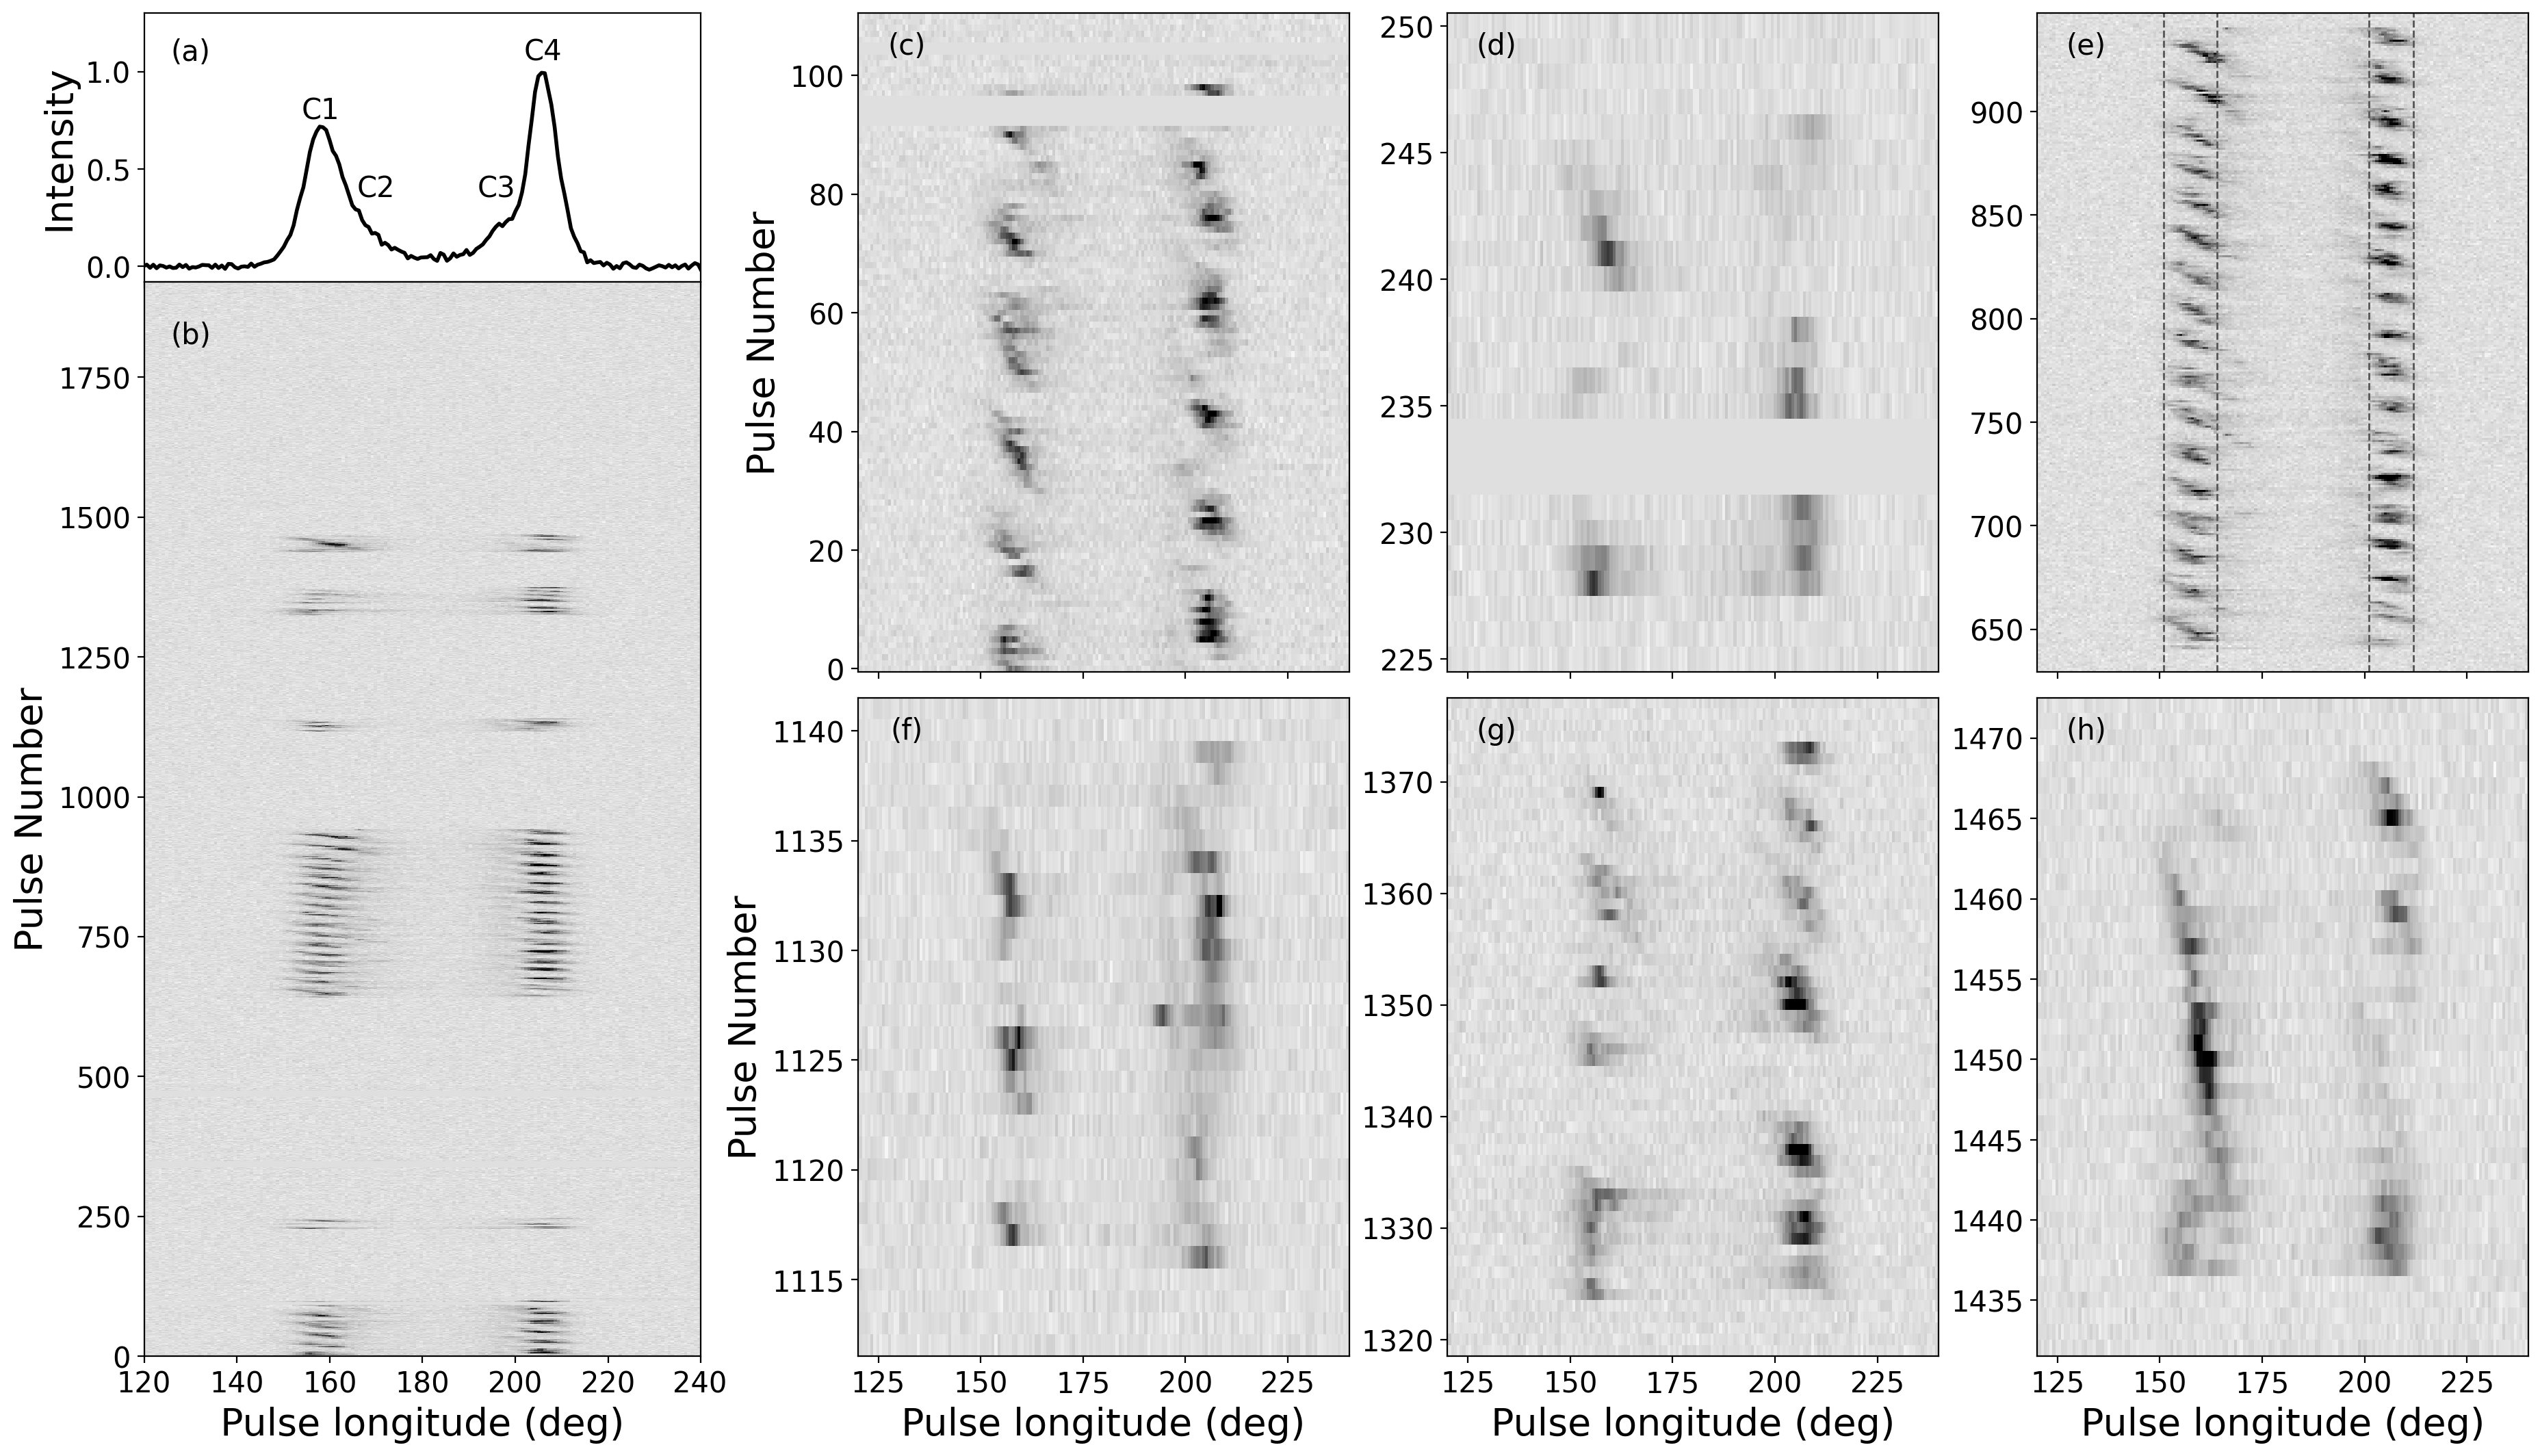
\includegraphics[height=0.8\textwidth]{Figures/J1926/stack.png}
            \caption[Pulse stacks of PSR~J1926$-$0652 as seen with FAST]{The integrated pulse profile of PSR~J1926$-$0652 averaged across the full 270 to 800~MHz band (panel (a)) with the four profile components labelled. The single pulses are shown in panel (b). The data shown is the single uncalibrated polarisation channel. Panels (c)--(h) show each of the six bursts present in the observation. The top three panels are bursts 1 to 3, and the lower panels are bursts 4 to 6.}
            \label{fig: J1926 - pulse stack}
        \end{center}
    \end{figure}
\end{landscape}
The pulsar clearly exhibits drifting subpulses, seen as diagonal intensity bands in the pulse stack, in all six bursts, which are of varying length. The longest is burst 3, which occurs between pulses 641 and 940 in the pulse stack. The overall profile width is approximately $60\degr$, and twin-peaked with a faint bridge of emission between the two components. Besides the bright pulse profile components (labelled C1 and C4 in the top left panel of Fig.~\ref{fig: J1926 - pulse stack}), there are also two fainter, blended nested components (C2 and C3) observed. These arise from the fainter emission on the inner edges of the bright driftbands -- C2 is very weak and appears to be a continuation of the driftbands giving rise to component C1, while C3, at slightly earlier longitudes than the C4 component, appears as a distinct shoulder in the average profile. The origin of these weaker components is most evident in burst 3, when the single pulse data is folded at the modulation period $P_3$ (see Sec.~\ref{sec: J1926 - analysis - P3 folding}).

An interesting observation is that in burst 3 (panel (e) of Fig.~\ref{fig: J1926 - pulse stack}) the separation between the two components appears to decrease along the burst, before resetting for bursts 4 to 6. It is not clear whether this behaviour is present in all bursts to different extents; a longer observation is needed to investigate this property. The most stable drifting subpulses occur in the longer bursts 1 and 3, whilst in the other bursts the drifting is highly irregular.

% The random noise in the off-pulse region where the no pulsar is present ought to have a mean level of zero. However, a variety of reasons can lead to a non-zero baseline. This has the potential to affect subsequent analysis as it may change throughout the pulse stack. Therefore, it is important to remove the baseline from the data, which is fairly simple as long as its variations are slow compared to the pulsar's period. Baseline subtraction for this data was done using the \texttt{pmod} tool in \textsc{psrsalsa} \citep{Wxxx2016}. To do this, a window is drawn over the region where signal from the pulsar can clearly be seen -- anything outside this region is assumed to be random noise, and the average of these samples can then be subtracted to give an off-pulse baseline with a mean of zero. When a given pulse is completely dominated by RFI, it is ``zapped'' (all intensity is set to zero) - several such pulses are visible in Fig.~\ref{fig: J1926 - pulse stack}.

When analysing the pulsar signal, the background level (which varies over time) should be subtracted. This is done by forcing the mean of the noise in the off-pulse region to be zero. THis baseline subtraction is fairly simple given the variations are slow compared to the pulsar's period, and has been done using the \texttt{pmod} tool in \textsc{psrsalsa} \citep{Wxxx2016}. The off-pulse region is identified by eye and the baseline is subtracted from each individual pulse separately. In addition, pulses which are completely dominated by RFI are ``zapped'' (all intensity is set to zero) -- several such pulses are visible in Fig.~\ref{fig: J1926 - pulse stack}.

\subsection{Fluctuation analysis}
\label{sec: J1926 - analysis - single pulse variability}


Fourier analysis can be used to quantify subpulse modulation. Two key techniques used in this analysis are the longitude-resolved fluctuation spectrum \citep[LRFS;][]{Bxxx1970a}, and the two-dimensional fluctuation spectrum \citep[2DFS;][]{ESxx2002}. The LRFS is used to detect periodicities that occur at a given pulse longitude across a pulse stack. If periodic modulation is occurring, a given column of intensities will resemble a sinusoidal pattern with a period $P_3$, which can be detected by performing discrete Fourier transforms (DFTs) in this direction. To calculate the LRFS, the pulse stack is divided into blocks of $n$ pulses where $n$ is the chosen length of the Fourier transform to be calculated. For each block, a DFT is calculated for each column corresponding to a fixed pulse longitude bin. The number of pulses in each block must be a power of two, and the length of the DFT determines the spectral resolution. The longer the block, the higher the resolution -- however, the signal-to-noise ratio (S/N) per spectral bin will decrease. Therefore a balance must be found. In this analysis, a block size of 512 pulses was used meaning only 1536 out of the 1921 total pulses in the FAST observation were used. As no emission was detected from pulse 1469 onwards, this does not affect the results. The power spectra for the individual blocks is then averaged to produce the LRFS, which has pulse longitude on the $x$-axis, and the periodicity $P_1/P_3$ in cycles per period (cpp) is displayed on the $y$-axis. 

Similar to the LRFS, the 2DFS highlights $P_3$ periodicities, and also $P_2$ periodicities. Additional Fourier transforms are calculated in the horizontal (pulse longitude) direction of the pulse stack in order to quantify any fluctuation that occurs \textit{within} a single pulse period, such as the separation between drifting subpulses. For this purpose $m$ on-pulse longitude bins are selected, where $m$ is once again a power of two. In the 2DFS, the vertical and horizontal directions correspond to $P_1/P_3$ and $P_1/P_2$ respectively. Asymmetry in fluctuation power with respect to $P_1/P_2 = 0$ would indicate that there is a preferred drift direction for the subpulses.

\begin{figure}
    \begin{center}
        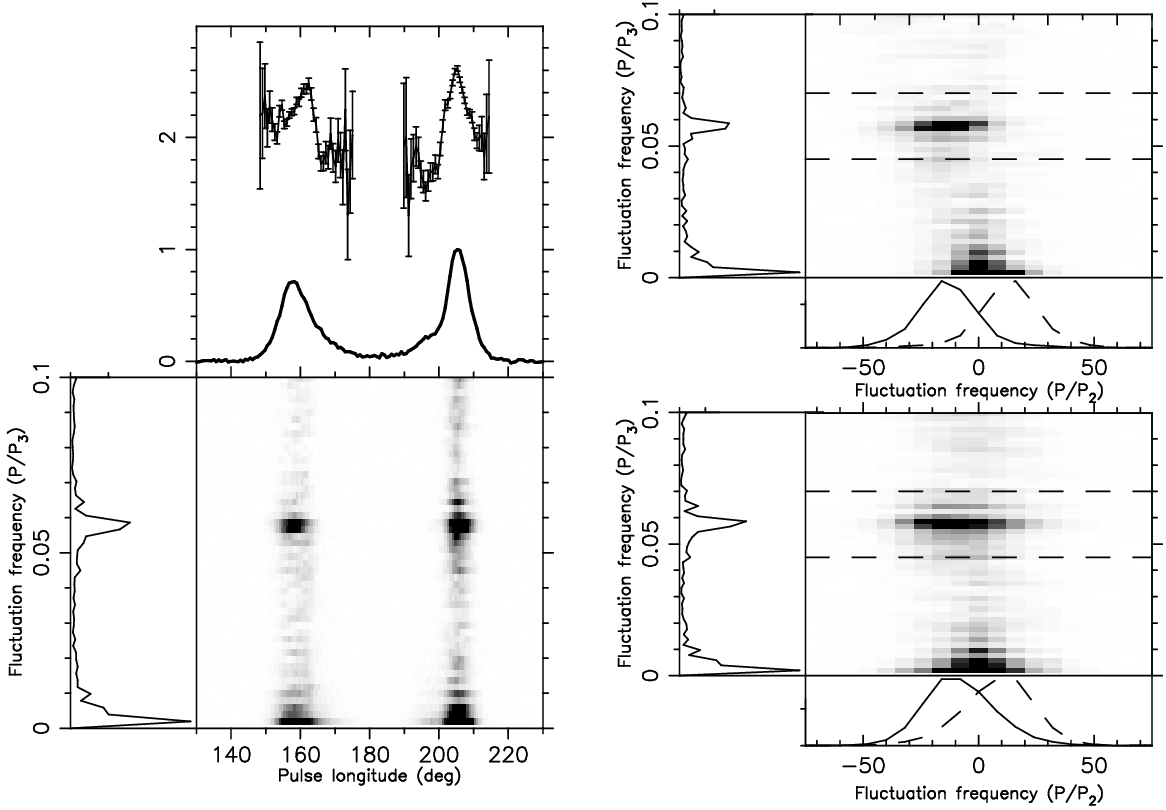
\includegraphics[width=1.0\textwidth]{Figures/J1926/fluctuation_spectra}
        \caption[LRFS and 2DFS of PSR~J1926$-$0652]{The fluctuation spectra for full FAST observation across the full frequency range of 270--800~MHz. The upper left panel shows the integrated pulse profile (solid line) and the longitude-resolved modulation index (black points with error bars). The lower left panel shows the LRFS, and the side panel is the result of integrating the power spectrum (greyscale) horizontally. The right-hand panels are the 2DFS for the leading components (upper plot) and trailing components (lower plot). Again, the left side panels of these are the result of integrating the power spectrum horizontally. The lower side plot shows the power spectrum integrated vertically between the two dashed lines (solid line). The dashed line in this panel shows the same distribution reflected about $P/P_2 = 0$ to highlight its asymmetry. Only part of the spectra are shown where the spectral features are strong ($0 \leq P_1/P_3 < 0.1$).}
        \label{fig: J1926 - fluctuation spectra}
    \end{center}
\end{figure}

Figure~\ref{fig: J1926 - fluctuation spectra} shows the fluctuation spectra for the full 270 to 800~MHz FAST observation of PSR~J1926$-$0652. The upper left plot shows the integrated pulse profile (solid line), along with the longitude-resolved modulation index (error bars). The modulation index is a measure of the variability of the intensity from pulse to pulse, and is equal to the standard deviation of the intensity divided by its the mean for a given pulse longitude bin. In this instance, the modulation index was calculated in the spectral domain alongside the LRFS and 2DFS, using the \texttt{pspec} program in \textsc{psrsalsa} \citep{Wxxx2016}. The error bars were calculated using bootstrapping, a robust statistical technique that requires no \textit{a priori} knowledge of the error distribution of the modulation index \citep[e.g.][]{WJxx2012}. In Fig.~\ref{fig: J1926 - fluctuation spectra} the modulation is strongest around the peak of the total intensity emission, close to profile components C1 and C4, and is slightly stronger in the latter. The displayed points are limited to those with a statistical significance greater than $3\sigma$. The modulation index is relatively large, and significantly larger than the modulation index shown in Fig.~B2 of \citet{ZLH+2019} which peaks at 1.3. This is because in Fig.~\ref{fig: J1926 - fluctuation spectra} the calculation of the modulation index includes the effect of nulls, while in the publication the spectra of burst 3 only were shown.

% Describe the LRFS plot
Periodicities in the single-pulse modulation can be quantified with fluctuation spectra. The lower left panel of Fig~\ref{fig: J1926 - fluctuation spectra} shows the LRFS, zoomed in to the on-pulse region between pulse longitudes $130\degr$ and $230\degr$. The greyscale plot shows the modulation power spectrum, and the left-hand side panel shows the spectrum integrated horizontally over the pulse window. There is a clear peak at $P_1/P_3 \simeq 0.058$~cpp for both the leading and trailing profile components, corresponding to the $P_3 \simeq 17 P_1$ periodicity in the driftbands which are clearly visible in the pulse stack (Fig.~\ref{fig: J1926 - pulse stack}). There is also an increase in spectral power visible towards $P_1/P_3 = 0$~cpp -- this is due to the nulls.

% Describe the 2DFS plots.
The two plots on the right hand side of Fig~\ref{fig: J1926 - fluctuation spectra} show the 2DFS, calculated separately for the leading half (components C1 and C2) and trailing half (components C3 and C4) in order to examine their drifting subpulses independently and to avoid the appearance of distortions in the spectra caused by non-linearity in how the driftbands in the two halves of the profile connect (see Sec.~\ref{sec: J1926 - analysis - phase tracks}). As with the LRFS, the features at $P_1/P_3 \simeq 0.058$~are clearly visible, and both have a clear offset from $P_1/P_2 = 0$ as highlighted in the lower line plots. In this panel, the solid line shows the power spectrum integrated vertically in the region of interest bounded by the horizontal dashed lines. In order to highlight the asymmetry of this distribution, it was reflected about $P_1/P_2 = 0$ and this is shown by the dashed line in the lower panels. The centroids of the spectral features were measured using the \texttt{pspecDetect} program in \textsc{psrsalsa} and the measured periodicities are $P_3 = (17.39 \pm 0.07)P_1$ and $P_2 = (25.5 \pm 0.4)\degr$ for components C1 and C2, and $P_3 = (17.33 \pm 0.09)P_1$ and $P_2 = (42\pm 1)\degr$ for components C3 and C4. These measurements are consistent with those presented in \citet{ZLH+2019} for burst 3 only. These values correspond to drift rates of $D = P_2 / P_3 = (1.47 \pm 0.02)\degr/P_1$ and $D = (2.42 \pm 0.06)\degr/P_1$ respectively. This quantifies the difference in the driftband gradients between the two halves of the profile that is clearly visible in Fig.~\ref{fig: J1926 - pulse stack}, especially for burst 3 (panel (e)). These values represent the \textit{average} drift properties across the full pulse stack -- the uncertainties quoted do not fully account for the large variability in the driftband shapes, or how they may change between different bursts. The lengths of the bursts are too short to reliably quantify their drift properties individually. The results for $P_3$ for the leading and trailing halves are consistent with one another, as expected if the drifting subpulses are produced by a circulating carousel (see Chapter~\ref{chapt: B0031}).




\subsection{\texorpdfstring{$P_3$}{P3} folding}
\label{sec: J1926 - analysis - P3 folding}

In order to more clearly see the average drift band structure in PSR~J1926$-$0652, the technique of $P_3$-folding was used, as described in Sec.~\ref{sec: intro - emission models - single pulse phenomena - P3 folding}. For PSR~J1926$-$0652, $P_3$ is highly variable, as can be seen in the irregular spacing of drift bands in bursts four to six in Figure \ref{fig: J1926 - pulse stack}. Burst 3 appears relatively stable and is the longest continuous time in which the emission was detected, and so this burst was chosen for $P_3$ folding. The last few driftbands were excluded as they have visually different shapes. As well as the full 270 to 800~MHz band, three frequency sub-bands spanning 270--400~MHz, 400--600~MHz, and 600--800~MHz were also analysed. A $P_3$ fold was formed for each sub-band as well as the full frequency range in order to study if and how the drift bands evolve with frequency. This was achieved by first folding the full frequency pulse stack with a periodicity $P_3 = 17.36P$ as this dataset has the highest S/N. Since $P_3$ is somewhat variable, phase offsets were allowed between blocks of 17 pulses. These phases, obtained by performing cross-correlations between the blocks of data, were recorded. The same phase offsets were used to fold the sub-band pulse stacks without doing any further fitting. In this manner, the $P_3$ folds are perfectly aligned and folded identically, permitting a meaningful comparison.

\begin{figure}
    \begin{center}
        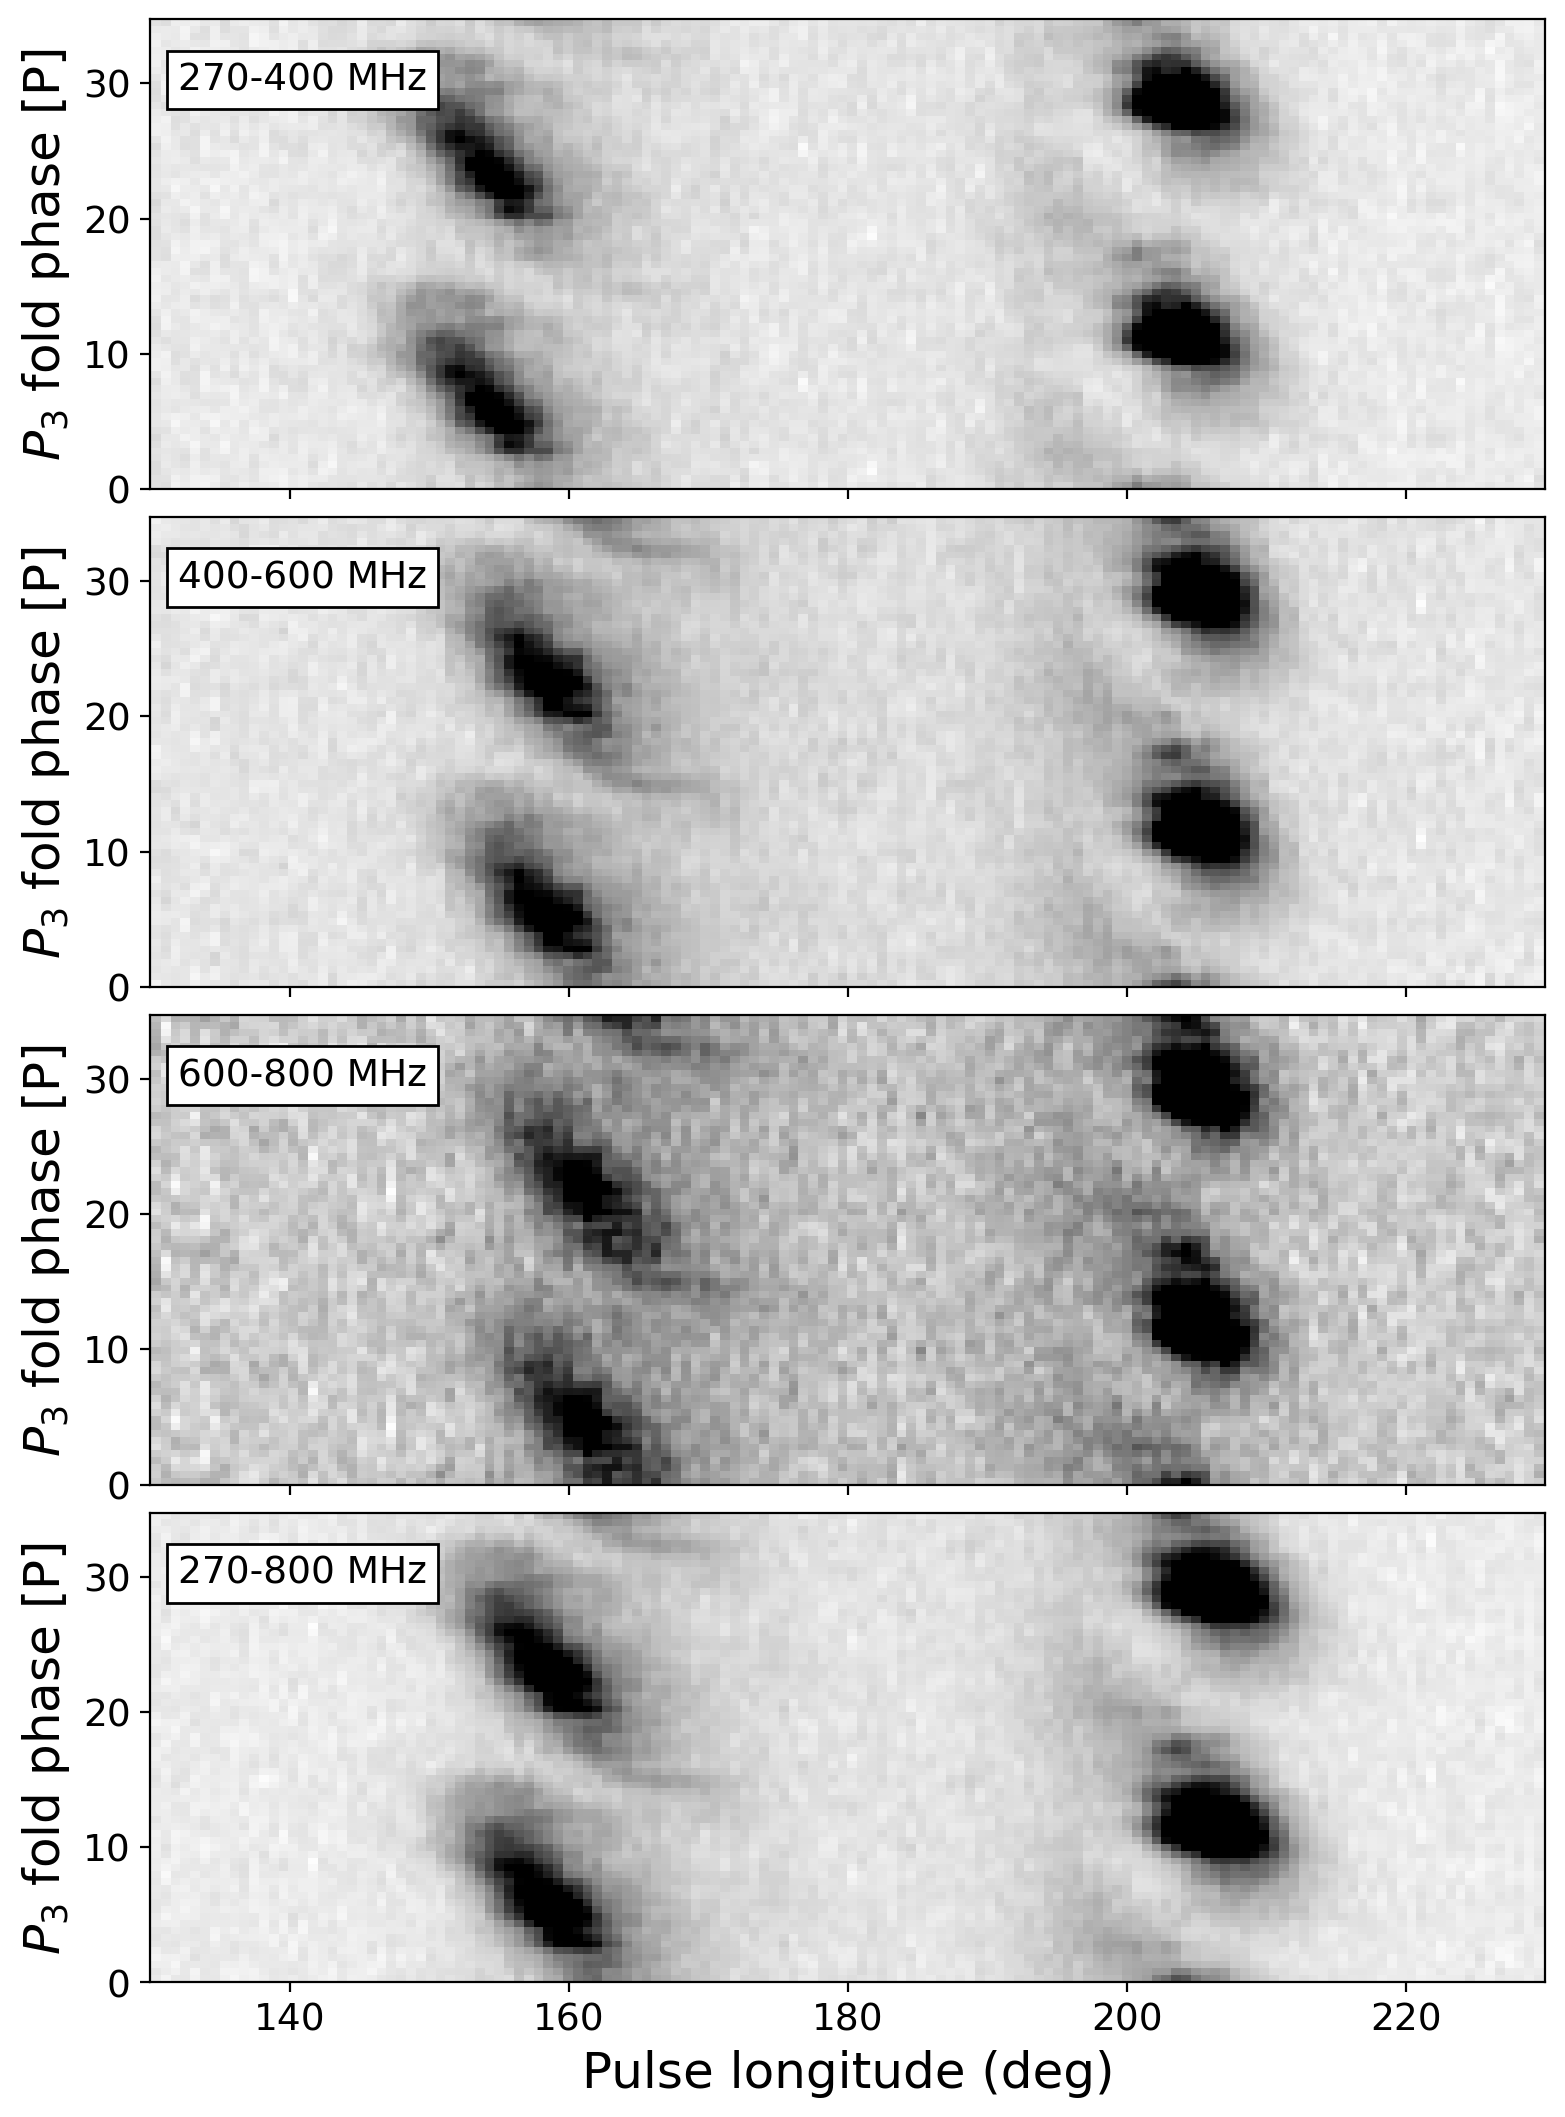
\includegraphics[width=0.8\textwidth]{Figures/J1926/p3_folds3}
        \caption[The average drift bands of PSR~J1926$-$0652 at different frequencies.]{A comparison of the average drift band obtained by $P_3$-folding the data of burst 3 at three different frequency bands. The top panel spans 270--400~MHz, the second panel spans 400--600~MHz, and the third panel spans 600--800~MHz. The bottom panel shows the average drift band across the combined frequency range of 270--800~MHz. The intensity has been clipped to 30~per~cent of its peak to highlight the fainter, inner structures.}
        \label{fig: J1926 - p3 folds}
    \end{center}
\end{figure}

The four $P_3$ folds are shown in Figure \ref{fig: J1926 - p3 folds}, with the bottom panel being identical to the $P_3$-fold shown in Fig.~B1 of \citet{ZLH+2019}. The sub-bands are plotted vertically beginning with the lowest frequency band at the top. The $P_3$ fold for the full frequency range is shown at the bottom. For clarity, each set of driftbands is plotted twice in order to show the continuity of the emission, and in order to better show the much weaker inner components the intensity has been clipped to 30~per~cent of its peak in each sub-band.  It is clear from the movement of the leading component to later pulse longitudes that the profile width decreases at higher frequencies, which is to be expected due to the narrowing of the emission region as described by radius to frequency mapping \citep[e.g.][]{Cxxx1978}. The two inner components (C2 and C3) are slightly more visible at higher frequencies, albeit still faint compared to the regions associated with profile components C1 and C4. In the leading half of the profile, the extra component appears as a small tail on the driftband at longitudes between $160\degr$ and $170\degr$ around a $P_3$-fold phase of 17, and is most visible in the 600--800~MHz sub-band -- this is component C2. Similarly an extension to the driftband appears in the trailing half, extending the emission to earlier pulse longitudes -- component C3. Here, the emission associated with C3 appears to be brightest between the main drift bands in $P_3$-phase, appearing between phases 17 and 26 at longitudes $195\degr$ and later. This discontinuity in the otherwise linear driftbands suggests that a single carousel is not enough to explain these observations. Subpulse phase tracks will be used next to quantify this discontinuity further. The analysis of the $P_3$ folds show that the profile shape is frequency dependent in terms of the both location of the components and their spectral indices.


% This apparent phase jump suggests an extra patch of emission may be responsible rather than a continuation of the main patch which forms the bright feature at $205\degr$. The $P_3$-folds provide one way of analysing the average drifting behaviour in PSR~J1926$-$0652, but are still confused by the presence of noise and bright features which dominate the low-intensity emission in the central bridge region. Therefore, an alternative analysis is required.


\subsection{Subpulse phase tracks}
\label{sec: J1926 - analysis - phase tracks}

The shape of the average driftbands can be quantified with the so-called subpulse phase as a function of pulse longitude. It is particularly useful in quntifying discontinuities and curvature in driftbands. The subpulse phase track follows from Fourier analysis, similar to that used to compute the LRFS and 2DFS (see Sec.~\ref{sec: J1926 - analysis - single pulse variability}). The pulse stack is divided into blocks of length defined by the length of the discrete Fourier transform (DFT) to be used. DFTs are calculated for each pulse longitude bin independently.

The DFT is calculated over a list of $N$ intensities $a_n$ according to
\begin{equation}
    A_k = \sum^{N-1}_{n=0} a_n e^{-i2\pi \frac{kn}{N}}.
\end{equation}
Here $N$ is the length of the DFT (the length of the block in the pulse stack, and a power of two), $n$ is the index of a given sample starting at $0$, and $k$ is the index of the corresponding sample in the resulting Fourier transform output ($0 \leq k \leq N/2$ \todo{CHECK}). The sequence $A_k$ is the DFT of the time series of flux densities $a_n$, where $A_k$ are complex numbers. Their amplitudes quantify how strong the frequency $k$ contributes to the signal, and the complex phase offset required to make a sinusoid with frequency $k$ match the time series. 

The modulation frequency $k$ is chosen to correspond to the $P_3$ period of the drifting subpulses as identified from the LRFS. The amplitude and complex phase of $A_k$ are calculated for all pulse longitudes independently. For linear driftbands the phase will change linearly with pulse longitude. We define the subpulses phase to have the opposite sign compared to the complex phase -- this ensures that an increasing subpulse phase with pulse longitude corresponds to positive drifting, i.e. subpulses that appear later at later longitudes. This means that the sight of the gradient of the subpulse phase track is identical to the gradient of the drifting subpulses in the pulse stack. Furthermore, the amplitude of $A_k$ can be considered as a function of pulse longitude, which quantifies how the intensity of the drifting subpulses change across the pulse window.

% discrete Fourier transform of the sequence $a_n$, each being a list of $N$ numbers. Each $A_k$ is a complex number. The amplitude corresponds to the strength of the modulation, and the phase corresponds to the phase of a sinusoid with frequency $k$ which matches the data.

% In practice, the modulation frequency $k$ is chosen by selecting a $P_3$ spectral bin of interest from the LRFS -- a sensible selection would be the peak value. The magnitude and phase of this modulation are calculated for all pulse longitudes independently. For linear driftbands the phase (subpulse phase) will change linearly with pulse longitude. Plotting the magnitude of the modulation as a function of pulse longitude gives an idea of how the driftbands change in intensity across the pulse window.

As well as burst 3 the most stable patterns of drifting occurs in burst 1, as can be seen in Fig.~\ref{fig: J1926 - pulse stack}. Bursts 1 and 3 lie within the pulse number ranges 0--94 and 641--930 respectively in the pulse stack, which means that the maximum FFT length for burst 1 is 64, and for burst 3 is 256. As shown earlier, the average modulation period for PSR~J1926$-$0652 is $P_3 = (17.4 \pm 0.1)P_1$ which corresponds to a frequency of $\sim$0.058~cpp. The closest spectral bin was selected for the two bursts.

\begin{figure}
    \begin{center}
        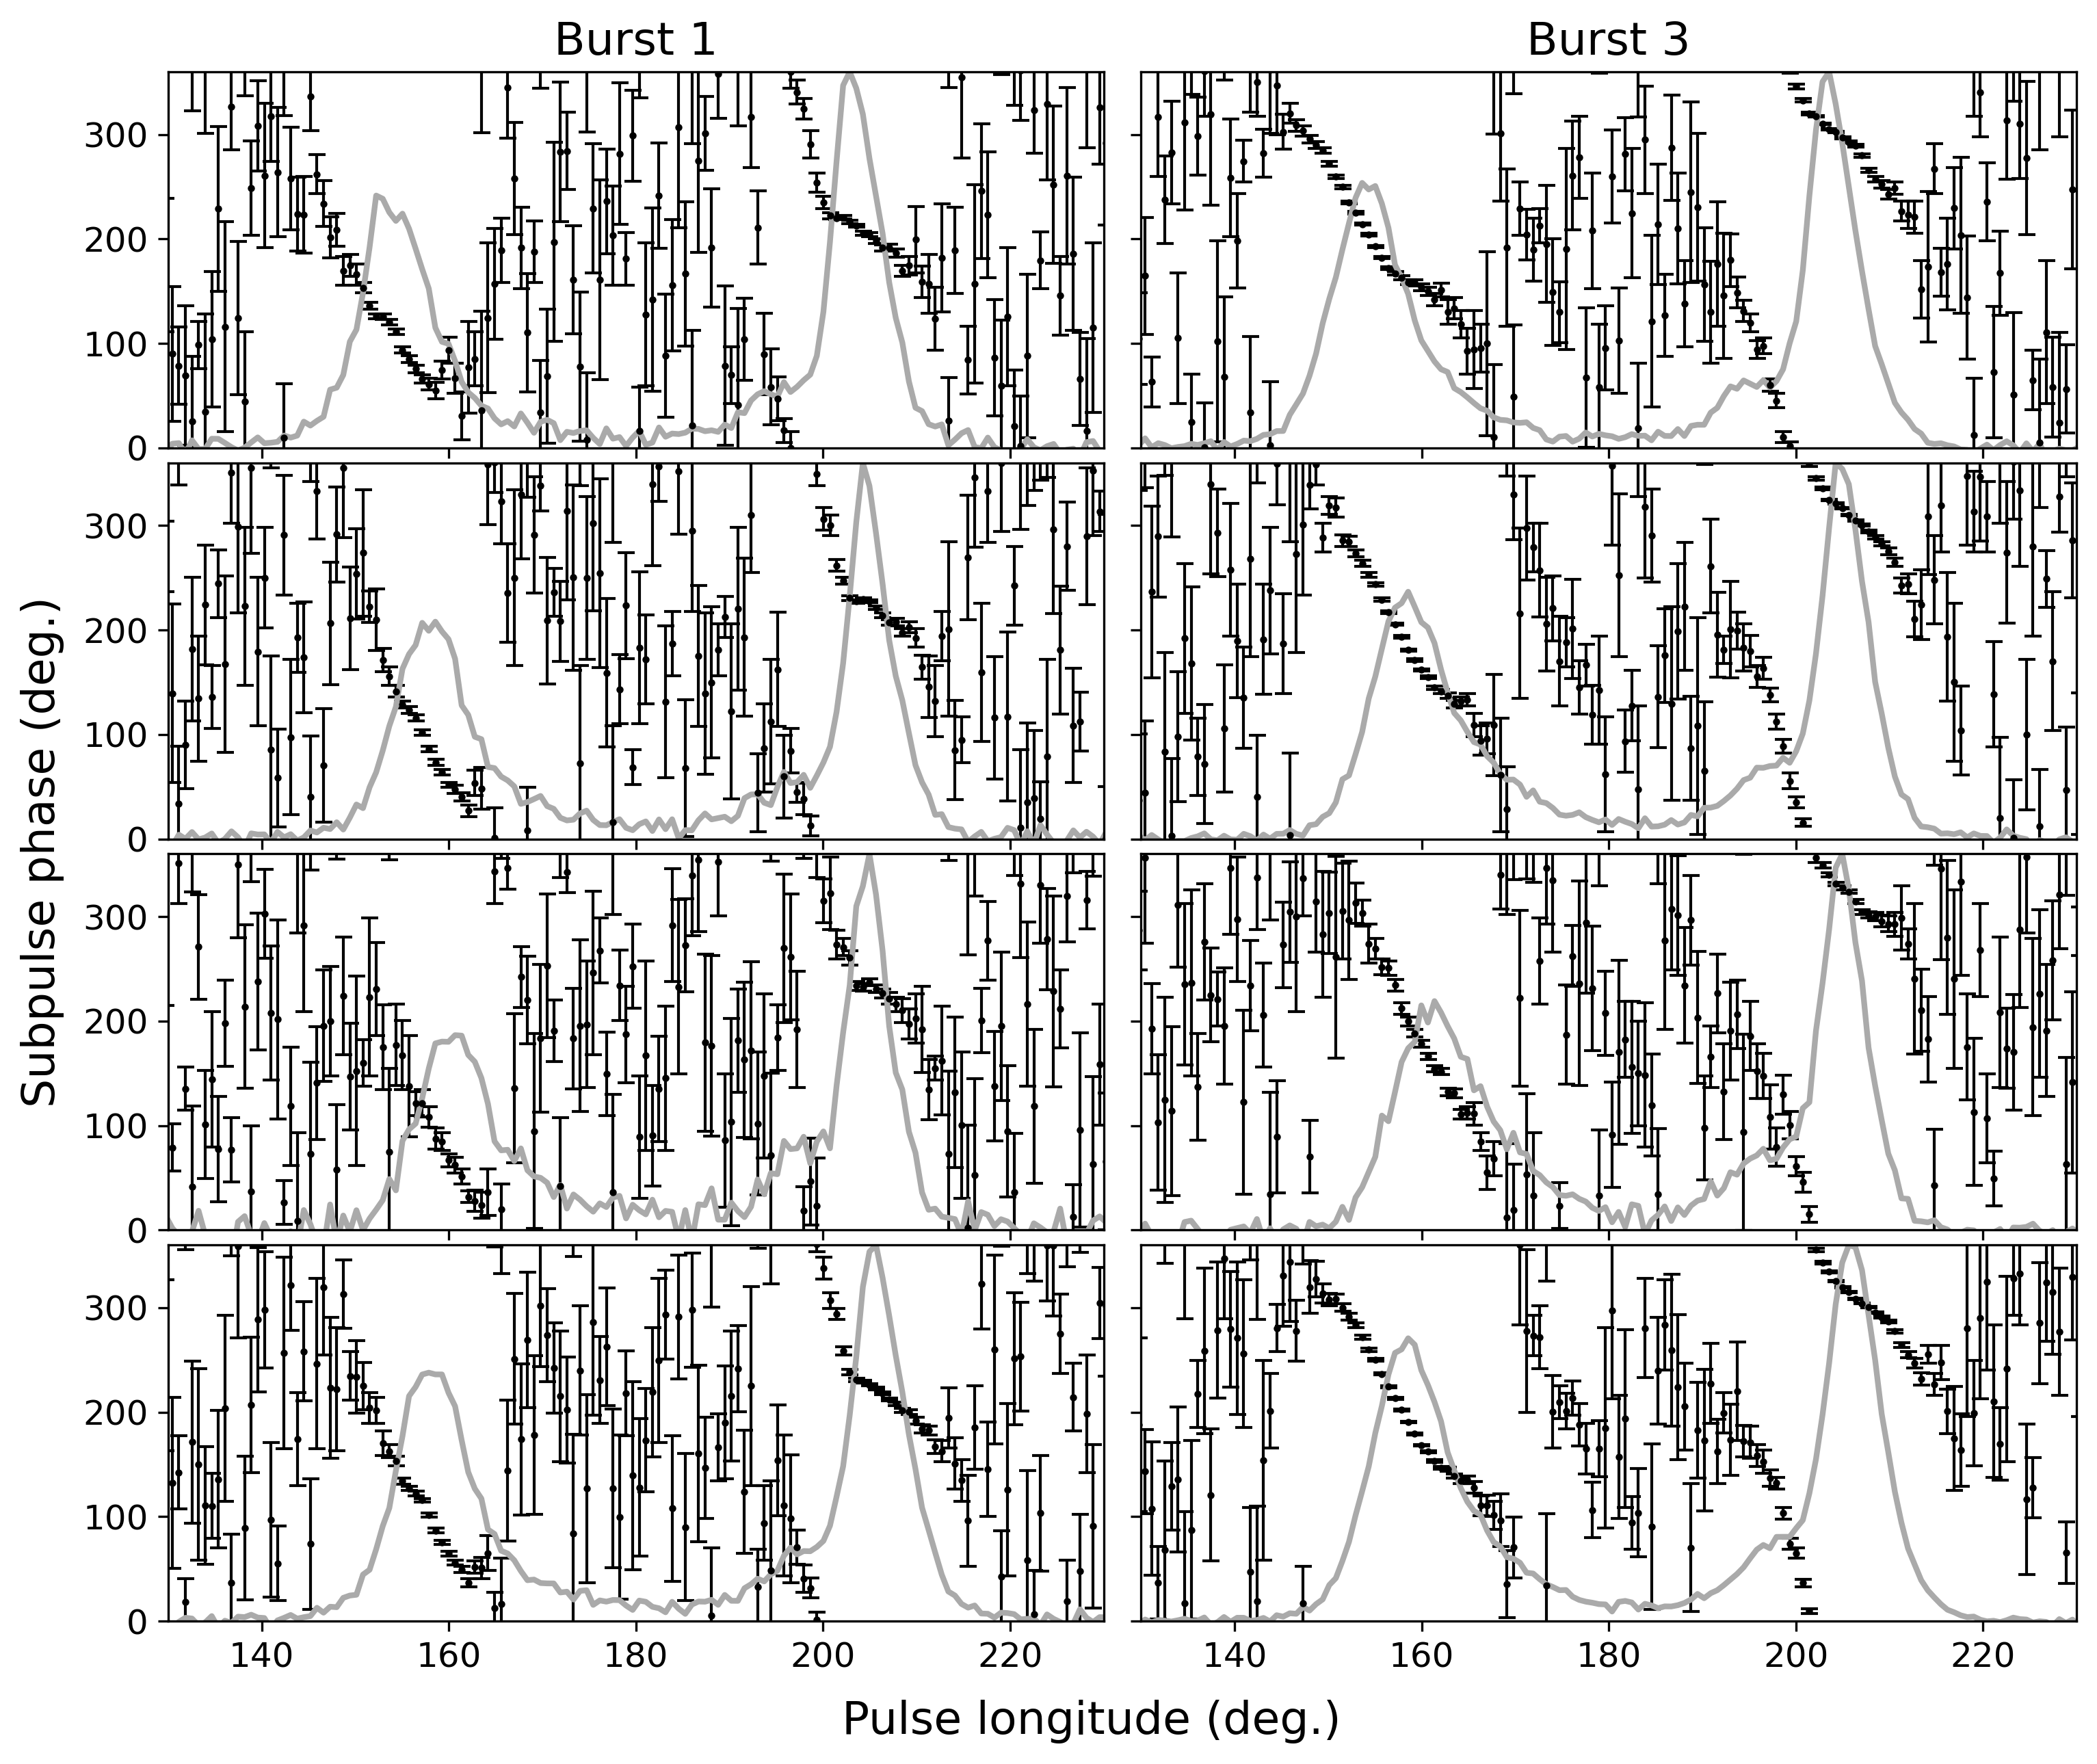
\includegraphics[width=1.0\textwidth]{Figures/J1926/subpulse_phase}
        \caption[Subpulse phase tracks PSR~J1926$-$0652]{A comparison of the subpulse phase tracks of bursts 1 (left column) and 3 (right column) at three different frequency bands. As for Fig.~\ref{fig: J1926 - p3 folds}, the top panels span 270--400~MHz, the second panels span 400--600~MHz, and the third panels span 600--800~MHz, while the bottom panels correspond to the entire frequency range of 270--800~MHz. The grey line shows the integrated profile for each burst at each frequency, while the black points with error bars show the longitude-resolved subpulse phase.}
        \label{fig: J1926 - phase tracks}
    \end{center}
\end{figure}

The subpulse phase tracks were calculated separately for each sub-band, for both burst 1 and burst 3 s shown in Figure~\ref{fig: J1926 - phase tracks}. The left hand column shows the results for burst 1, and the right shows the results for burst 3. As in Fig.~\ref{fig: J1926 - p3 folds}, the sub-bands are shown in order of increasing frequency with the 270--400~MHz band at the top. The bottom row shows the results for the full frequency range of 270--800~MHz. Within each panel the integrated profile for the burst is shown by the pale grey line. The subpulse phase track is shown by the black points with error bars. These error bars were calculated using bootstrapping, where white noise was added to the data with a standard deviation determined from the off-pulse region for each dataset. The phase track was recalculated for one thousand iterations. For each pulse longitude there is then a distribution of subpulse phases; the standard deviation of these was taken as the uncertainty on the measurement.

For both bursts broadly similar results are obtained, although burst 3 has an overall higher S/N because of its greater length. In the leading half of the profile the phase track is continuous and reasonably straight, with an almost constant negative gradient. Towards lower frequencies a slight kink becomes visible at $\sim$150$\degr$, coinciding with the peak of the C1 profile component. The kink appears to occur earlier than the boundary between the C1 and C2 components. In contrast, the phase track in the trailing half of the profile shows a distinct discontinuity in its gradient at the boundary between the C3 and C4 profile components. In the pulse longitude range associated with C4 the phase track has a gradient comparable to that of the leading half, with a steepening gradient towards the trailing shoulder of the profile. However, at the earlier longitudes corresponding to the C3 profile component the gradient of the phase track is considerably steeper. The track wraps fully around the phase boundary at $360\degr$, which implies that for some pulses two subpulses corresponding to successive driftbands are observable. This can indeed be seen in Fig.~\ref{fig: J1926 - p3 folds}. \todo{The steeper portion of the track appears to be out of phase with the track in the leading half of the profile by approximately $90\degr$.} Some structure is faintly visible in the bridge region, although the uncertainties on these points are much higher. Discontinuities in phase tracks have previously been seen in other pulsars -- their interpretation is discussed in Sec.~\ref{sec: J1926 - discuss - phase track}.
















\subsection{Polarisation properties}
\label{sec: J1926 - analysis - polarisation}

The follow-up data from the Parkes telescope in Australia, which was used for long term timing of PSR~J1926$-$0652, could be used to perform reliable polarimetric analysis. The calibrated data of the different observations were summed to create a polarised integrated profile using the \textsc{psrchive} software \citep{HSMx2004} and this was then further analysed using \textsc{psrsalsa}. The program \texttt{ppol} was used to calculate the polarised profile shown in Figure \ref{fig: J1926 - parkes profile}.
\begin{figure}
    \begin{center}
        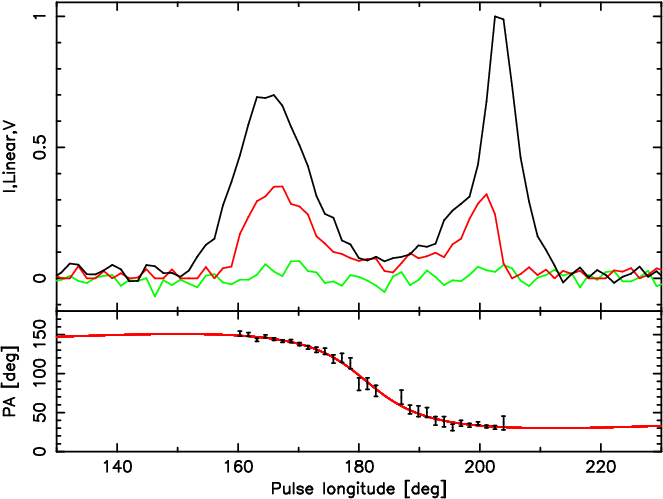
\includegraphics[width=0.6\textwidth]{Figures/J1926/parkes_profile}
        \caption[Polarised profile of PSR~J1926$-$0652 observed with Parkes]{The polarised profile of PSR~J1926$-$0652 as it was observed with the Parkes telescope. In the upper panel the black, red, and green lines show the total intensity, linear polarisation, and circular polarisation respectively. In the lower panel the points show the PA as a function of pulse longitude, fitted by the RVM (red curve).}
        \label{fig: J1926 - parkes profile}
    \end{center}
\end{figure}
In the upper panel the normalised total intensity $I$ profile is shown by the solid black curve, and the linearly polarised intensity $L$ is shown by the red curve. There is a negligible amount of circularly polarised emission $V$, as indicated by the green line. The fractional linear polarisation is moderate at $(38\pm1)$~per~cent which was de-biased according to \citet{WKxx1974}, and there is little evidence for significant circular polarisation. The lower panel shows the position angle of linear polarisation (PA) as a function of pulse longitude (black points). The uncertainty on the PA arises from the measurement errors on the Stokes parameters, which are Gaussian-distributed with equal standard deviations such that $\sigma_I = \sigma_Q = \sigma_U = \sigma_V$. The PA is given by $\psi = 0.5\arctan(U/Q)$ (see Sec.~\ref{sec: intro - emission models - polarisation}), so from standard error propagation its uncertainty is
\begin{equation}
    \label{eq: J1926 - PA uncertainty}
    \sigma_\psi = \frac{1}{2L^2}\sqrt{U^2\sigma_Q^2 + Q^2\sigma_U^2},
\end{equation}
where $L^2 = Q^2 + U^2$. \todo{AGREE IT'S ODD TO SHOW EQ WITH DIFFERENT SIGMAS AFTER SAYING THEIRY EQUAL, BUT NOT SURE WHAT ELSE TO DO, OTHER THAN REMOVE THE EQUATION?} In reality the errors on $\psi$ are non-Gaussian due to its cyclic nature, and so normal error propagation is not strictly valid -- this was explored in detail by \citet{NCxx1993}. Equation~\eqref{eq: J1926 - PA uncertainty} is a good approximation if $L$ is highly significant; in Fig.~\ref{fig: J1926 - parkes profile} the displayed PA points are limited to those in which $L$ is at least twice the off-pulse rms of $I$, and so the calculated uncertainties are reliable.

As explained in Sec.~\ref{sec: sec: intro - emission models - polarisation - RVM}, according to the Rotating Vector Model (RVM) the PA  in radio pulsars is indicative of the orientation of the magnetic field lines where the emission was produced. The RVM predicts the PA to have a characteristic S-shaped curve as a function of pulse longitude. The RVM is parametrised by the magnetic inclination angle, $\alpha$, and line-of-sight impact parameter $\beta$ with respect to the magnetic axis, and has an inflection point at ($\phi_0$, $\psi_0$). In full,
\begin{equation}
    \tan(\psi - \psi_0) = \frac{\sin(\phi-\phi_0)\sin\alpha}{\sin(\alpha+\beta)\cos\alpha-\cos(\alpha+\beta)\sin\alpha\cos(\phi-\phi_0)}.
    \label{eq: J1926 - RVM}
\end{equation}

Fitting Eq.~\eqref{eq: J1926 - RVM} to the observed PA was achieved by performing a grid search over $\alpha$ and $\beta$, and then optimising the free parameters $\psi_0$ and $\phi_0$ by minimising the $\chi^2$ fit of the observed PA. A second program from {\sc psrsalsa}, \texttt{ppolFit} was used to achieve this. The parameters $\phi_0$ and $\psi_0$ were initially estimated by eye from the shape of the PA curve, and then optimised using the downhill simplex method \citep{PTVF2007}. This minimisation process was then repeated across the grid of $\alpha$ and $\beta$ values. The optimum fit is shown as the red curve in the bottom panel of Fig.~\ref{fig: J1926 - parkes profile} which is a good fit to the data, confirmed by the reduced-$\chi^2$ of 0.8.
\begin{figure}
    \begin{center}
        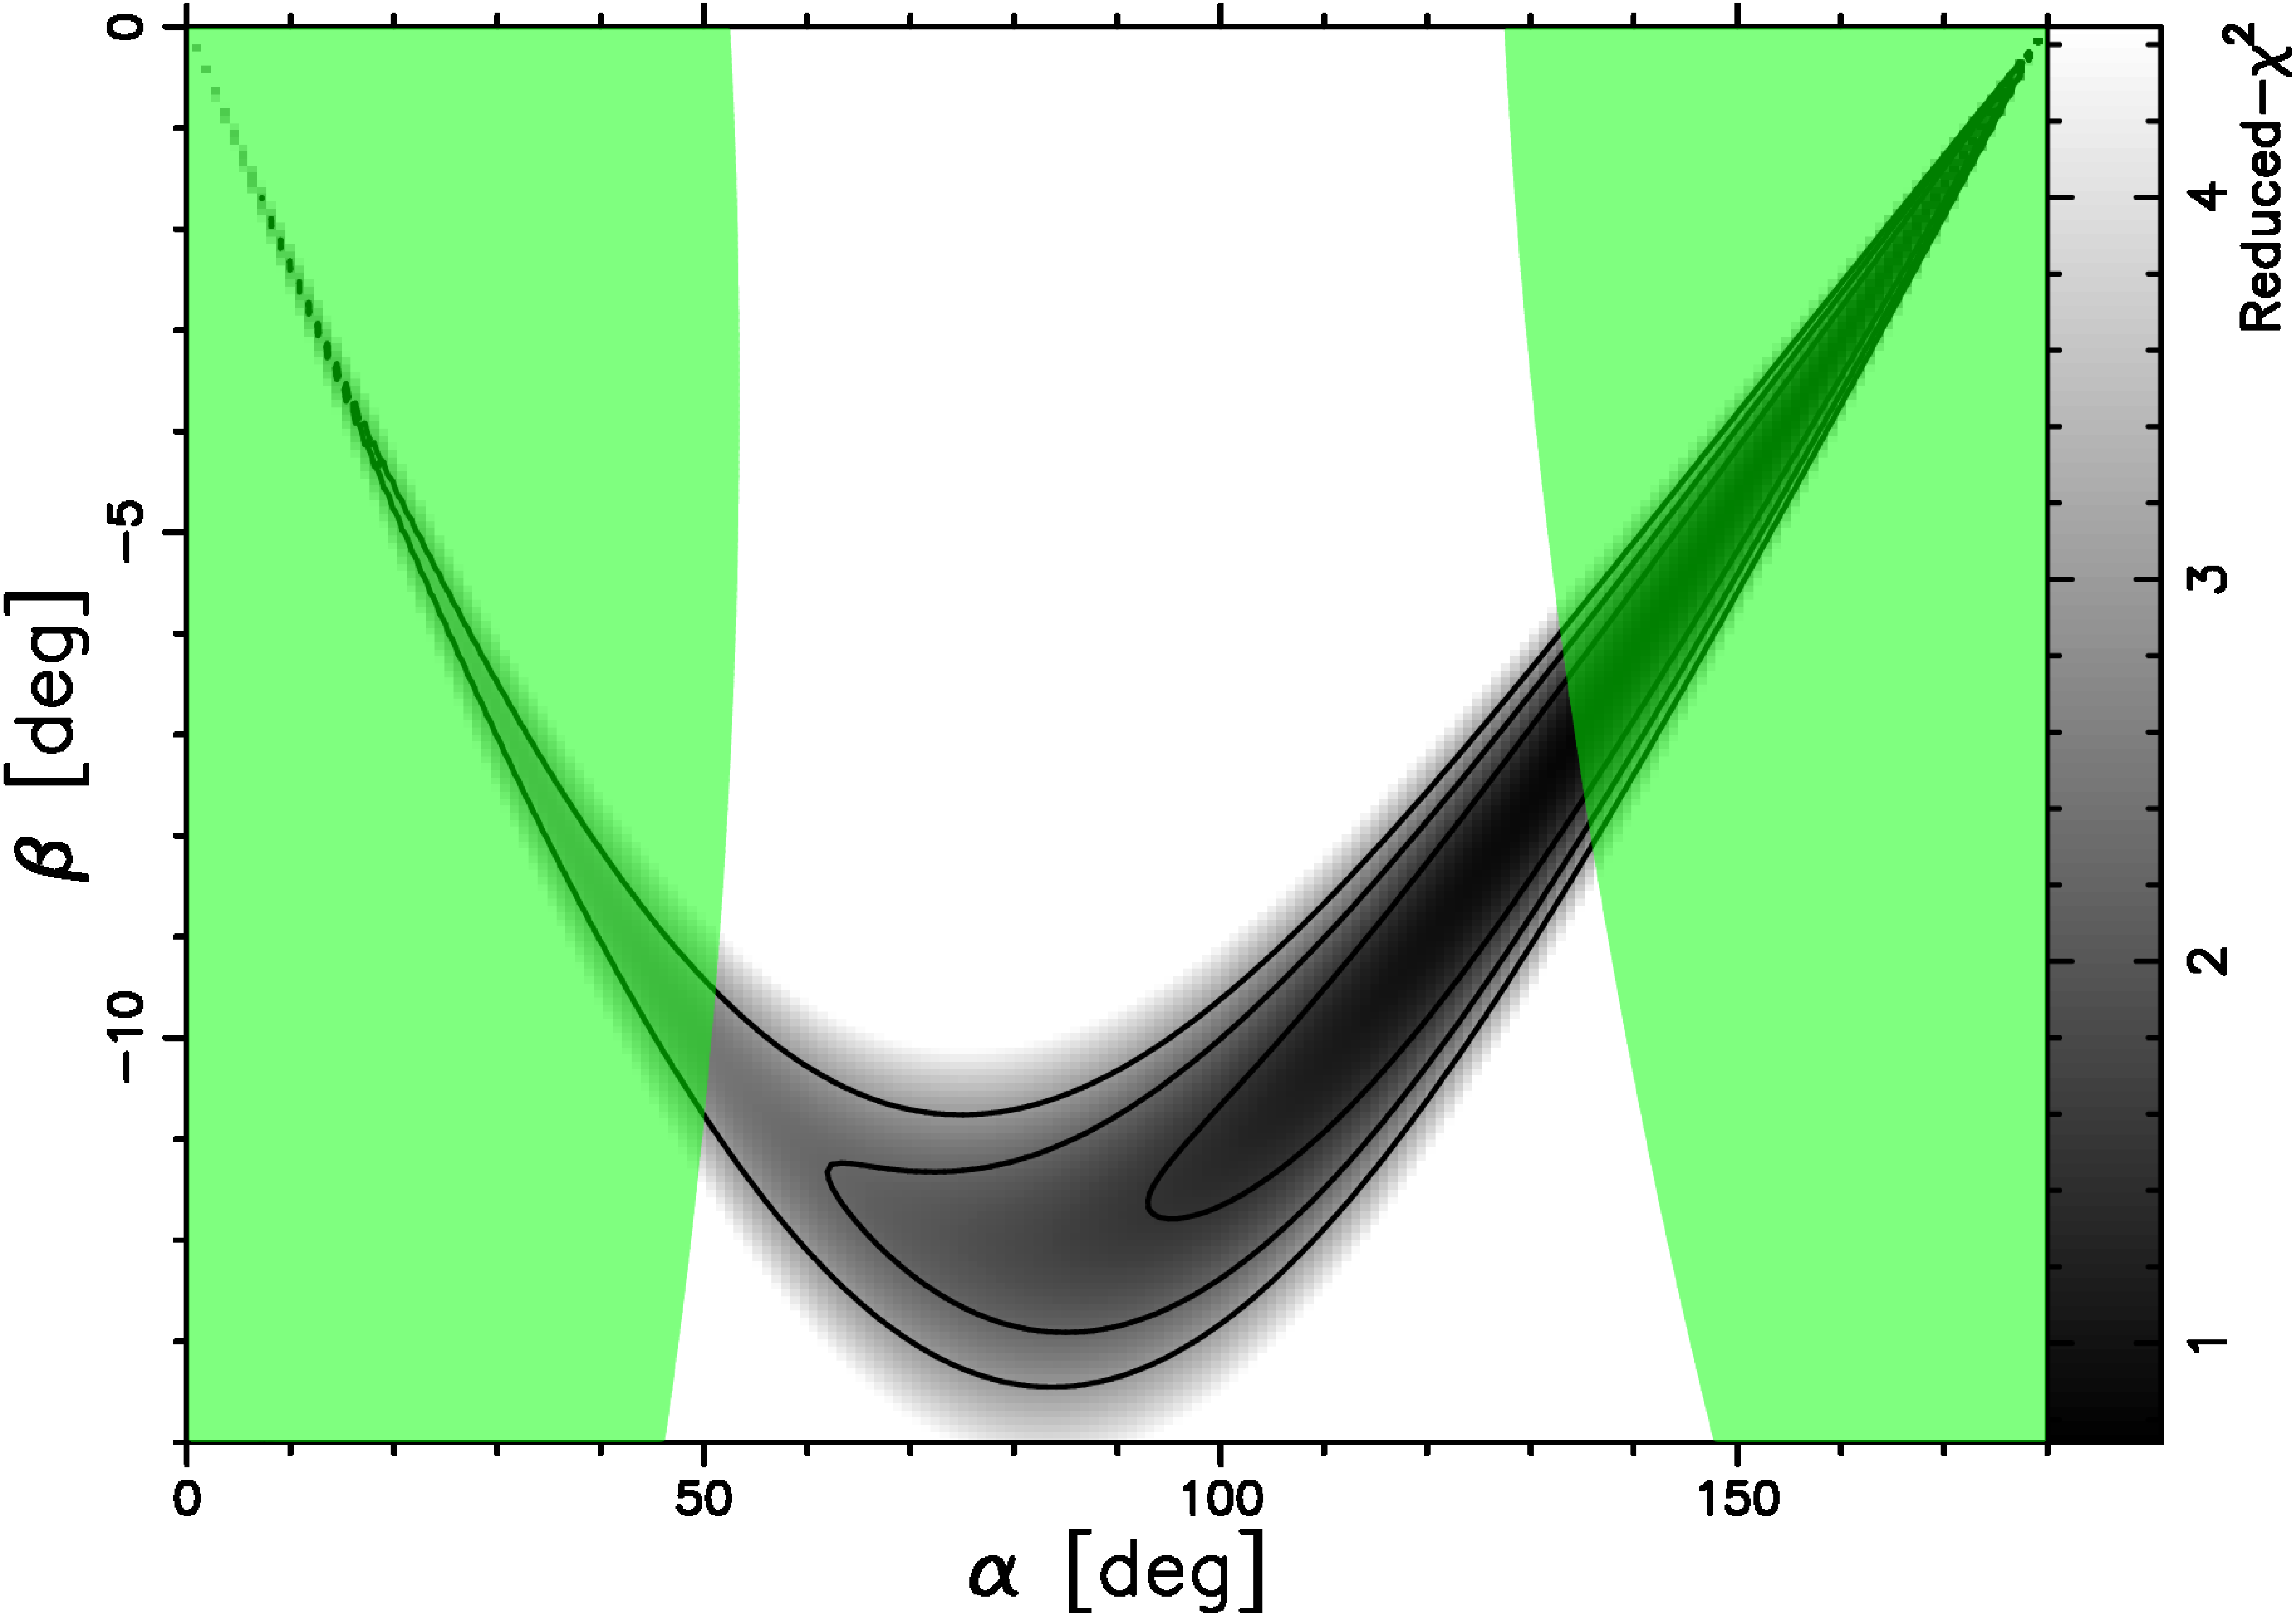
\includegraphics[width=0.6\textwidth]{Figures/J1926/banana_plot}
        \caption[The goodness-of-fit of the RVM to the PSR~J1936$-$0652 PA curve]{The results of fitting the RVM across a grid of $\alpha$ and $\beta$ values. The greyscale indicates the reduced-$\chi^2$. The contour lines represent $1\sigma$, $2\sigma$, and $3\sigma$ confidence intervals corresponding to two, three, and four times the lowest reduced-$\chi^2$. The green regions indicate ``allowed geometries'' based on the observed profile width.}
        \label{fig: J1926 - banana plot}
    \end{center}
\end{figure}

There is no single solution of the RVM that fits the data satisfactorily, as shown by the distribution of reduced-$\chi^2$ across ($\alpha$, $\beta$) space (Fig.~\ref{fig: J1926 - banana plot}). This shows that despite the fit being very good, $\alpha$ is practically unconstrained by the RVM. The impact parameter is constrained to $|\beta| \lesssim 14^\circ$.

Further constraints can be placed upon the viewing geometry by taking into account the observed profile width, using the method of \citet{RWJx2015a}. The width of the pulse profile is governed by how the observer's line of sight (LOS) intersects the emission beam, which is determined by $\alpha$ and $\beta$. \citet{GGRx1984} showed that the pulse longitude range $W$ (the pulse width) for which the LOS intersects the open-field-line region is given by 
\begin{equation}
    \label{eq: J1926 - allowed geometry}
    \cos\rho = \cos\alpha\cos(\alpha+\beta)+\sin\alpha\sin(\alpha+\beta)\cos\bigg(\frac{W}{2}\bigg),
\end{equation}
where $\rho$ is the half opening angle of the cone of radio emission. The opening angle of the emission cone is delimited by tangents to the last open field lines at the height at which emission is produced, $h_\mathrm{em}$. However, it should be noted that the open field line region does not necessarily produce emission over its full extent \citep[e.g][]{LMxx1988}, and so the measured profile width may not necessarily correspond to the full extent of the open field line region. In the small angle limit \citep[i.e. $h_\mathrm{em} \ll R_\mathrm{LC}$, e.g.][]{Rxxx1990}, the half opening angle of this cone defined by the open field line region is given by
\begin{equation}
    \label{eq: J1926 - emission cone angle}
    \rho = \sqrt{\frac{9\pi h_\mathrm{em}}{2cP}}.
\end{equation} 
The combination of Eqs.~\eqref{eq: J1926 - allowed geometry} and \eqref{eq: J1926 - emission cone angle} implies that for a given $\alpha$ and $\beta$, pulsars with a greater emission height will produce wider profiles because of the diverging dipole field with emission height. The emission height also has an effect on the polarisation properties of the pulse profile, through relativistic aberration and retardation (A/R) effects which cause the inflection point of the RVM curve (Eq.~\eqref{eq: J1926 - RVM}) to move to later pulse longitudes, whilst the total intensity profile appears to shift earlier. \citet{BCWx1991} showed that the expected delay in pulse longitude between the fiducial plane and the RVM inflection point is $\Delta\phi = 4h_\mathrm{em}/R_\mathrm{LC}$, where $R_\mathrm{LC}$ is the size of the light cylinder (see Sec.~\todo{INTRODUCTION SECTION}). By measuring this delay, the emission height can be estimated.

As seen in Fig.~\ref{fig: J1926 - parkes profile}, the inflection point of the RVM curve fitted to the PA data lies close to the centre of the profile of PSR~J1926$-$0652, which has a ``single cone'' morphology \citep[][]{Rxxx1983a}. The shift due to A/R effects is believed to be no more than $\sim$14$\degr$, implying an emission height of less than 5000~km. From Eq.~\eqref{eq: J1926 - emission cone angle}, $\rho < 22.4\degr$. The relatively large observed width of the profile at 10~per~cent of the peak intensity was taken to be $W_{10} = 61\degr\pm 4\degr$. The green areas in Fig.~\ref{fig: J1926 - banana plot} indicate which values of $\alpha$ and $\beta$ are able to produce a profile of the measured width according to Eq.~\eqref{eq: J1926 - allowed geometry}, given the upper limit on emission height. These ``allowed geometries'' moderately constrain $\alpha \lesssim 55\degr$.





\subsection{Nulling in \texorpdfstring{PSR~J1926$-$0652}{PSR~J1926--0652}}
\label{sec: J1926 - analysis - nulling}
Even in this short observation PSR~J1926$-$0652 exhibits frequent nulls of different lengths as seen with FAST, with a nulling fraction of approximately 75~per~cent over this short observation. Although the nulls are generally obvious in the pulse stack (Fig.~\ref{fig: J1926 - pulse stack}) and take place over tens to hundreds of periods, a short null of four pulses may also have occurred in the middle of burst 5, between pulse numbers 1341 and 1344 (inclusive). Figure~\ref{fig: J1926 - burst five null} highlights the pulses in question.
\begin{figure}
    \begin{center}
        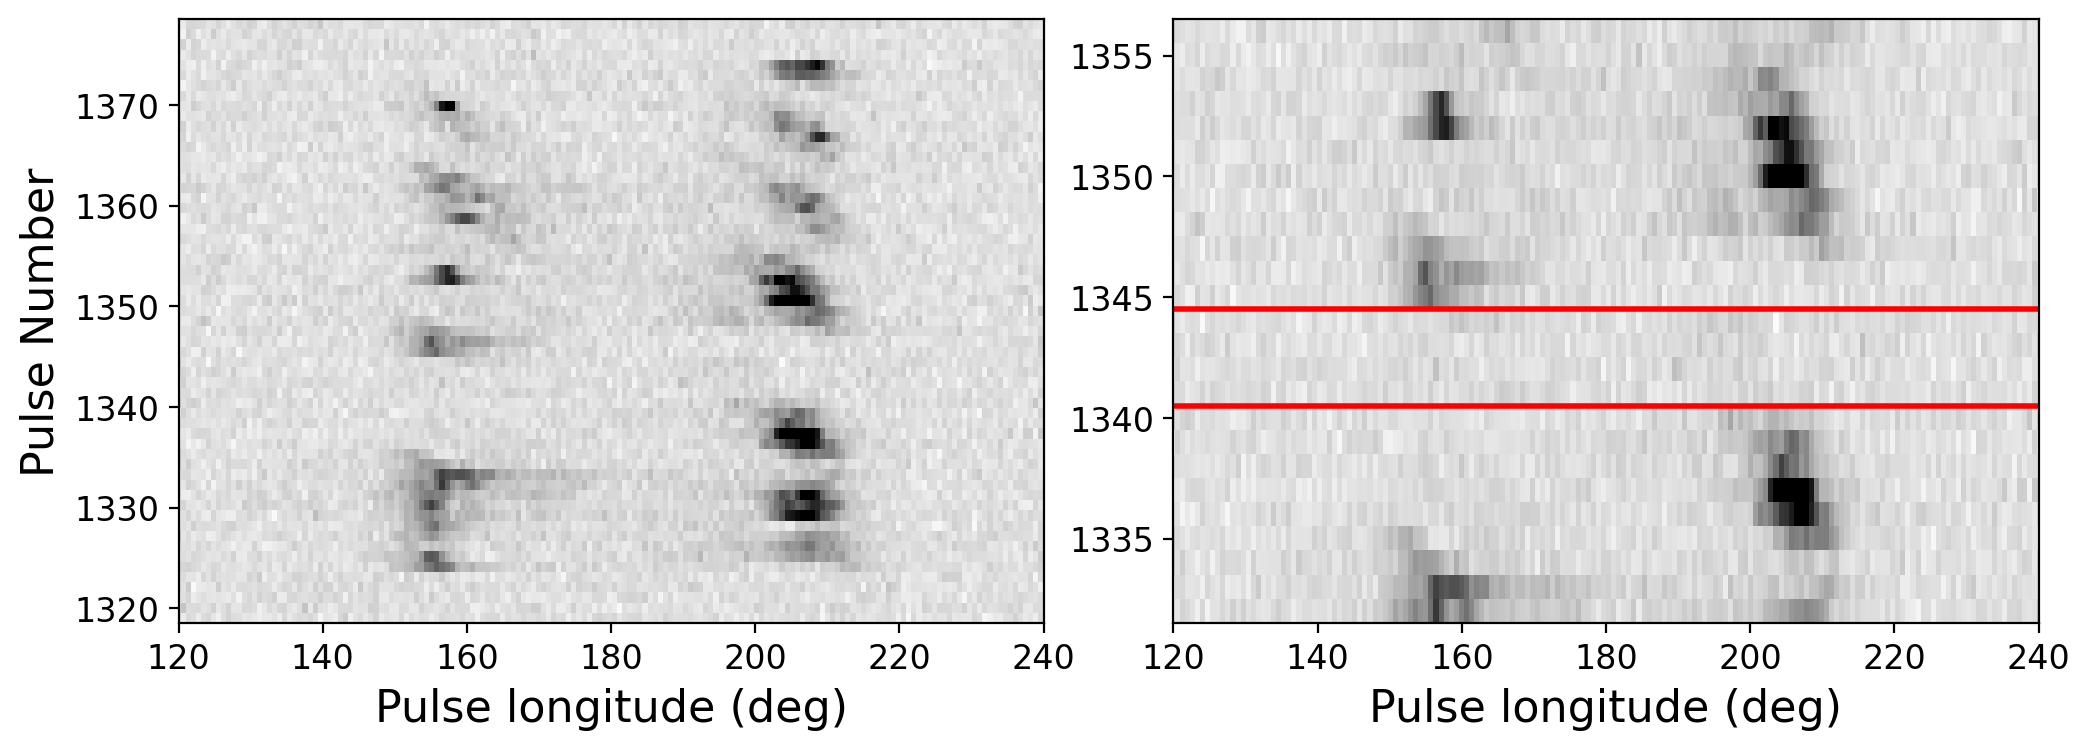
\includegraphics[width=1.0\textwidth]{Figures/J1926/burst_5}
        \caption[Burst 5 of PSR~J1926$-$0652 showing the possible null]{The single pulses observed with FAST, showing burst five. The red lines in the right-hand panel enclose those pulses for which no emission was detected in either component. It is unclear whether this is an example of a short null, or if this feature is due to the erratic drifting behaviour observed in this and the other short bursts.}
        \label{fig: J1926 - burst five null}
    \end{center}
\end{figure}
For these four rotations no emission integrated over the nominal pulse width is detected, with an upper limit of $5\sigma_\mathrm{pe}$ where $\sigma_\mathrm{pe}$ is the expected uncertainty based on the noise observed in the off-pulse region. 
However, given the separation between the driftbands $P_3 \simeq 13P_1$, which moreover is clearly variable, it is  difficult to say for sure whether this is a true null or is simply part of the erratic drifting subpulse pattern as seen in the shorter bursts (see bursts 2, 4, 5, and 6 in Fig~\ref{fig: J1926 - pulse stack}).

As is the case for the potential null shown in Fig.~\ref{fig: J1926 - burst five null} and most of the clearer nulls, the leading half of the profile appears to disappear first. The ``last active pulses'' (LAPs) in the pulse stack before a null are shown in Fig~\ref{fig: J1926 - LAP and FAP profiles}. The ``first active pulses'' (FAPs) after a null are also shown. 
\begin{figure}
    \begin{center}
        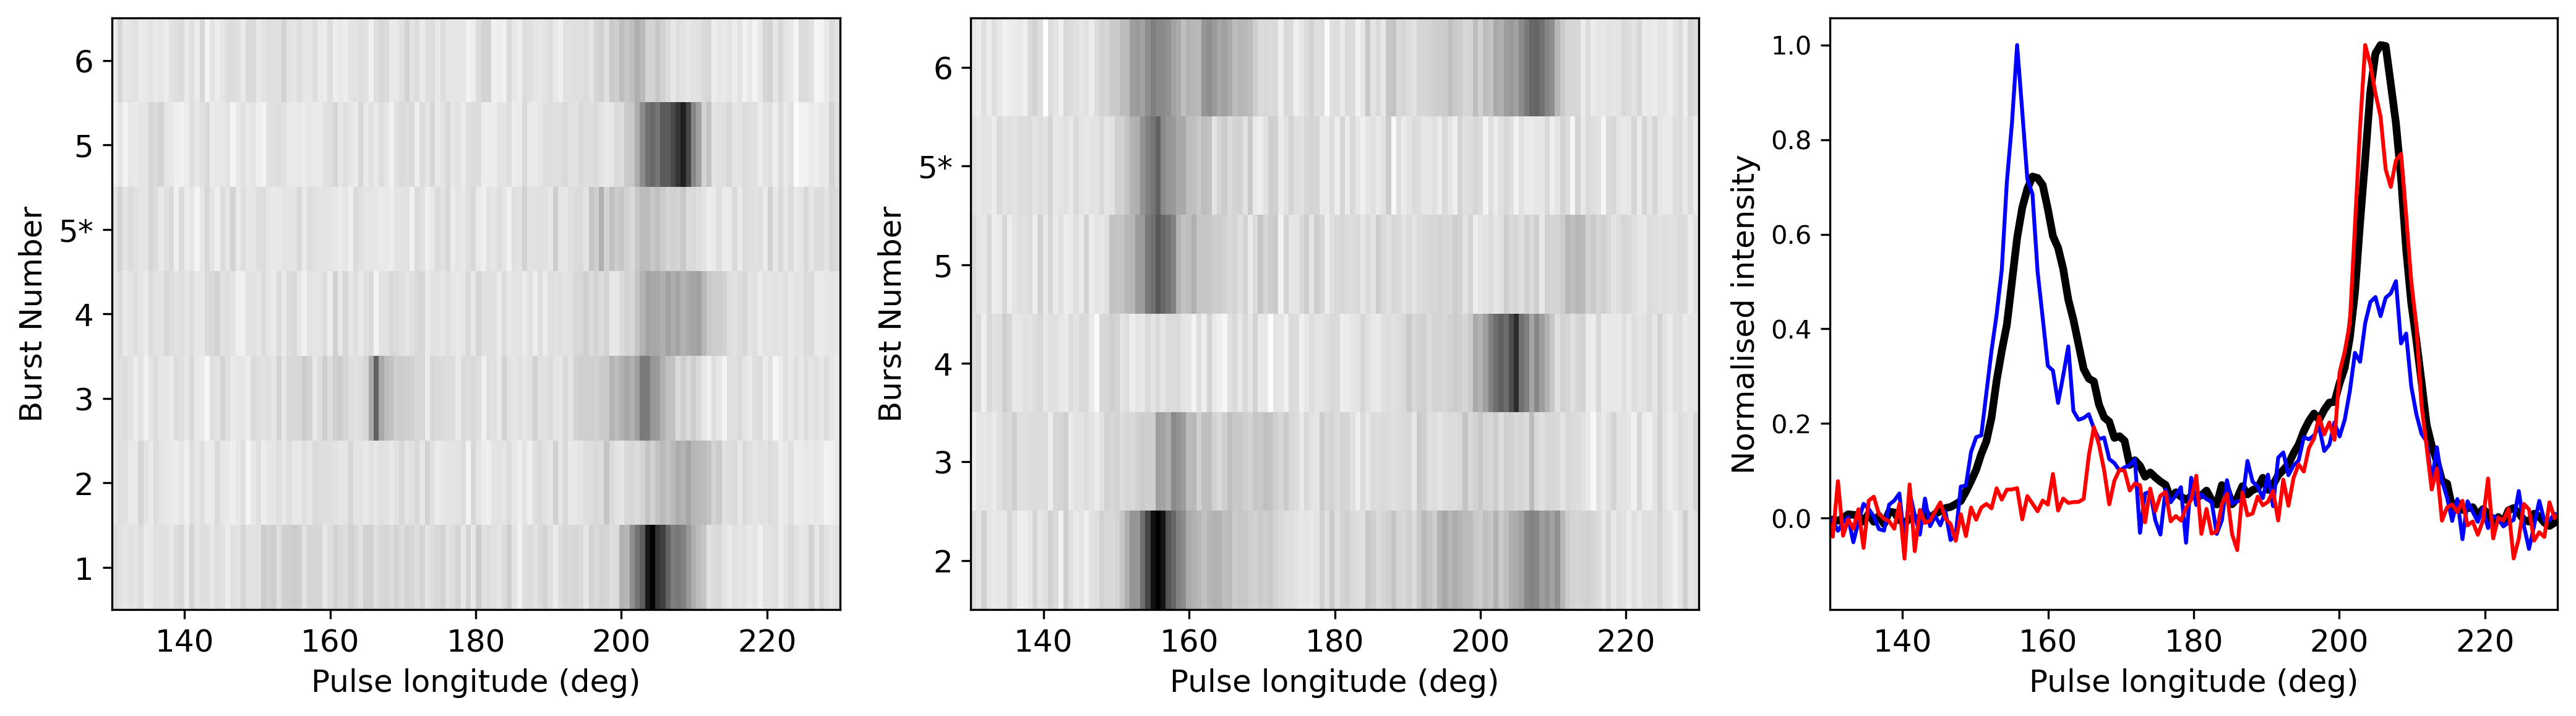
\includegraphics[width=1.0\textwidth]{Figures/J1926/LAPFAP_profiles}
        \caption[Comparison of LAP and FAP to integrated profile]{The intensities of the individual LAPs (left panel) and FAPs (centre panel). The pulses for the bursts labelled ``5*'' correspond to the potential null in burst 5. The right-hand panel shows a comparison of the integrated profile of the full pulse stack (black line) to the integrated profiles of the LAPs (red) and the FAPs (blue). The profiles have been normalised to their respective peak intensities. }
        \label{fig: J1926 - LAP and FAP profiles}
    \end{center}
\end{figure}
There are seven LAPs shown in the left-hand panel, corresponding to the last pulses of bursts 1--6, and also including the potential short null in burst 5 -- this is labelled as burst 5*. There are only six FAPs however -- this is because at the start of the FAST observation PSR~J1926$-$0652 is already in its ``on'' state, so the FAP of burst 1 was not recorded. The LAPs and FAPs were summed to create an integrated profile for each set. These are shown in the right-hand panel of Fig.~\ref{fig: J1926 - LAP and FAP profiles} alongside the integrated profile for the entire pulse stack for comparison (thick black line). The LAP and FAP profiles are shown by the thinner red line and blue curves respectively.

The individual LAP pulses and their profile show very clearly that the leading components of the profile are distinctly weaker just before the pulsar enters the null state. The ratio between the leading and trailing profile components is extreme, far greater than in the overall average profile. A difference is also seen in the FAP profile, although the difference compared to the overall pulse profile is less extreme. The disappearance of the leading components immediately prior to a null suggests a link between the phenomenon of nulling and drifting subpulses. If the drifting subpulses are produced by sub-beams arranged in a circulating carousel pattern (see Chapter~\ref{chapt: B0031}), that would require the sub-beams to extinguish in a very specific sequence related to their circulation. This will be discussed further in Sec.~\ref{sec: J1926 - discuss - LAP}.

Very few bursts of emission were observed by FAST, and the pulse shapes are highly variable, meaning that the difference between the LAP, FAP, and overall pulse profile might not be significant. The question we considered is ``if the pulsar enters and leaves a null state at a random time (i.e. a random phase in the $P_3$ cycle), how likely is it to observe a LAP/FAP profile constructed from a few pulses which is extreme as what is observed?''.
To quantify this, seven and six pulses (which corresponds to the number of LAP and FAP pulses respectively) were selected at random from all ``on'' state pulses (excluding the actual LAP and FAP pulses), and summed to create an integrated profile. From this profile the strengths of the leading and trailing profile components were calculated by integrating the flux density in their respective peaks, and the ratio $R$ was computed. This process was repeated 500,000 times. The results are shown in Fig.~\ref{fig: J1926 - LAP and FAP histograms}.


This ratio as determined from the observed LAP and FAP profiles (red and blue curves respectively in the right-hand panel of Fig.~\ref{fig: J1926 - LAP and FAP profiles})is $R=0.154$ and $1.302$.  For comparison, the integrated profile for the full pulse stack is $R = 0.896$.
\begin{figure}
    \begin{center}
        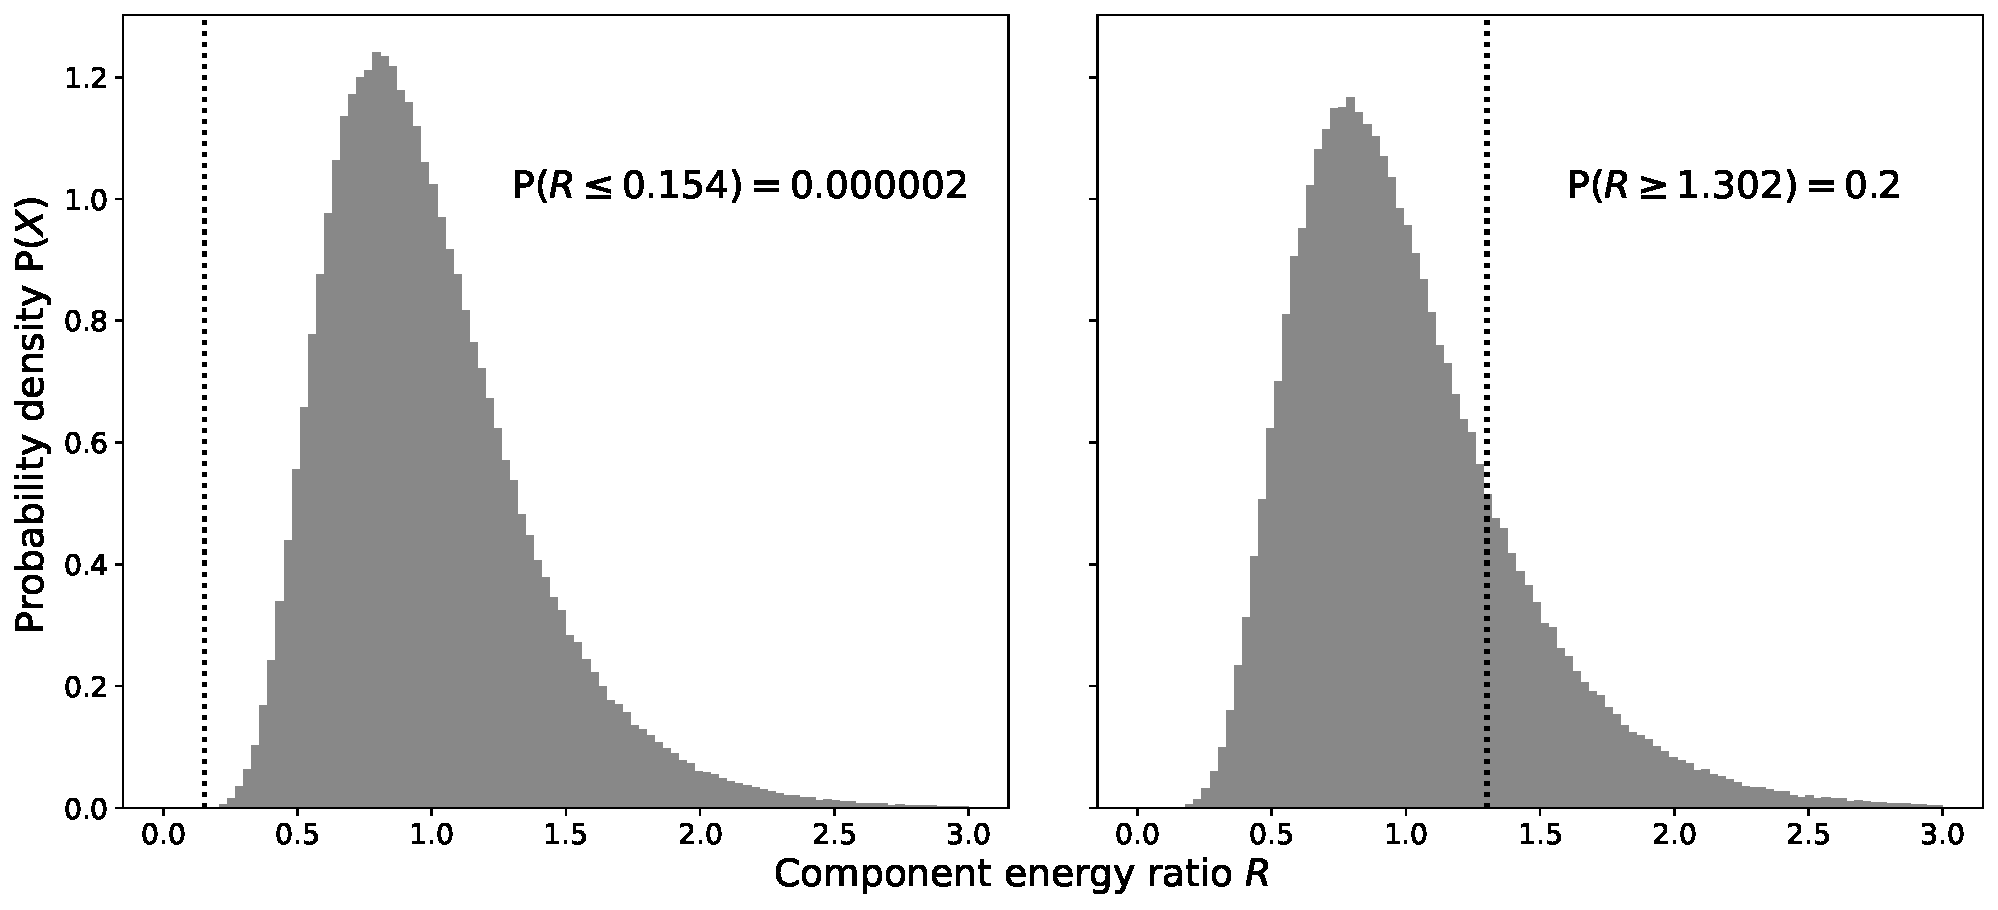
\includegraphics[width=0.9\textwidth]{Figures/J1926/LAPFAP_histograms}
        \caption[Calculating the significance of the LAP and FAP profiles]{Histograms showing the distribution of the peak power ratio of 500,000 randomly created integrated profiles corresponding to the LAPs (left panel) and FAPs (right panel). The vertical dashed lines indicate the measured ratio of the real integrated LAP (left) and FAP (right) profiles.}
        \label{fig: J1926 - LAP and FAP histograms}
    \end{center}
\end{figure}
Of the 500,000 trials, only one resulted in $R$ more extreme than that measured for the actual LAP profile. Therefore this difference between the LAP profiles and the overall profile is highly significant. In contrast, 99,980 randomised FAP profiles (20~per~cent) had a ratio $R$ greater than the observed FAP profile, so this is not significant given the low number of nulls recorded.
In this analysis it was assumed that the four off-state pulses in burst 5 (Fig.~\ref{fig: J1926 - burst five null}) should be considered to be a null. If this is \textit{not} the case, $R$ would be 0.176 for the LAP profiles and the probability for this to occur at random would be $P(R\geq 0.176) = 0.003$, making the LAP profile still a $3\sigma$ outlier. We have therefore shown that there is a connection between the drifting subpulses and the time at which PSR~J1926$-$0652 enters a null, which will be discussed further in Sec.~\ref{sec: J1926 - discuss - LAP}.



















\section{Discussion}
\label{sec: J1926 - discussion}

\subsection{Profile and geometry}
\label{sec: J1926 - discuss - geometry}

The integrated pulse profile of PSR~J1926$-$0652 has four components: two bright, primary components (C1 and C4); and two somewhat dimmer, inner components (C2 and C4). There is also a bridge of weak emission connecting the leading and trailing components. The overall structure is a twin-peaked profile. Various models of the emission region have been put forward to explain the variety of profile shapes seen in the population (see \citealt{KJxx2007} for a full review and empirical model) -- these include the core-cone model \citep[e.g.][]{Rxxx1983a, Rxxx1986}, and the ``patchy beam'' of \citet{LMxx1988}. This work does not explicitly rule out any beam model; however, the fact that drifting subpulses are observed in the leading and trailing components means that it is likely that profile shape arises from the line of sight intercepting a ring of circulating sub-beams arranged in a carousel structure. This is further discussed in Sec.~\ref{sec: J1926 - discuss - phase track}.

The profile becomes narrower with increasing frequency, as demonstrated by Fig.~\ref{fig: J1926 - p3 folds}. This is a commonly observed phenomenon \citep[e.g.][]{CWxx2014,PHS+2016}, and is the expected behaviour if the higher frequencies are produced at lower altitudes in the magnetosphere, where the open field line region is narrower \citep[e.g.][]{RSxx1975,KGxx2003}. In Fig.~\ref{fig: J1926 - p3 folds} it appears as though the narrowing of the profile is caused by the movement of the leading profile components to later pulse longitudes while the trailing component remains at a constant phase. However, this behaviour depends on the choice one makes for the dispersion measure (DM; see Sec.~\ref{sec: intro - observation processing - ISM effects - dispersion}). The figure is for a DM$= 84.7 \pm 0.9\ \mathrm{cm}^{-3}\mathrm{pc}$ \citep{ZLH+2019}. This choice of DM follows from optimising the overall S/N of the integrated pulse profile. This optimisation will attempt to align the pulse profile as a function of frequency after removal of the frequency-dependent dispersive delay. However, if the profile itself is frequency-dependent, it is difficult to disentangle the two contributions. This is illustrated in Fig.~\ref{fig: J1926 - dedispersion}.
\begin{figure}
    \begin{center}
        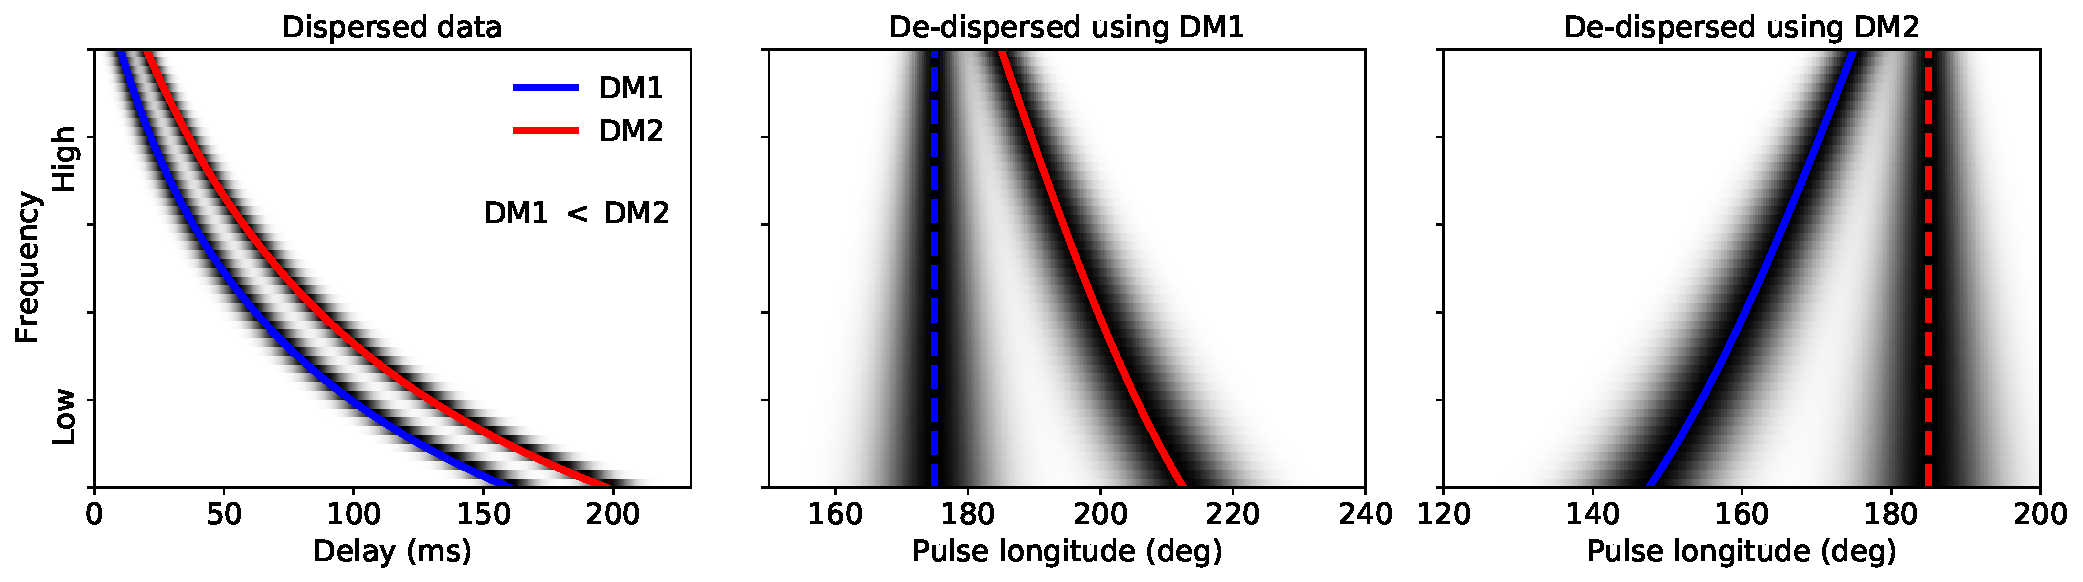
\includegraphics[width=1.0\textwidth]{Figures/J1926/dedispersion_demo}
        \caption[Ambiguity in de-dispersion of a multi-component pulse profile]{An illustration of the ambiguity encountered when de-dispersing data for a pulsar with a twin-peaked profile. The components of the profile move closer together at higher frequencies, meaning that two slightly different DMs may be measured in the frequency-resolved dispersed data (left panel). The blue and red lines correspond to the peak of each component as a function of frequency. Due to the changing position of the components a DM optimising the S/N of the earlier component (DM1) will be slightly smaller than the DM optimising the S/N of the trailing component (DM2). De-dispersing using DM1 will lead to the leading component remaining stationary in pulse phase while the trailing component appears to shift to earlier longitudes at higher frequencies (centre panel), while de-dispersion using DM2 will lead to the opposite (right panel).}
        \label{fig: J1926 - dedispersion}
    \end{center}
\end{figure}
De-dispersing with different DMs may either align one or the other component across the frequency band, whilst the other appears to change pulse longitude. It is likely that the profile of PSR~J1926$-$0652 narrows with increasing frequency, which would mean both components move inwards rather than one component being stationary.

The Parkes telescope data of PSR~J1926$-$0652 shows that it is fit very well by the RVM (see Fig.~\ref{fig: J1926 - parkes profile}). Despite the excellent fit, the magnetic inclination angle $\alpha$ remained unconstrained. Further constraints were applied based on the observed profile width, which is reasonably broad spanning $\sim$60$\degr$ pulse longitude, suggesting that $\alpha \lesssim 55\degr$. A broad profile can occur in two ways: if the emission is produced at high altitudes, in which case the emission cone formed by the tangents to the last open field lines will be very wide; or if $\alpha$ is small in which case the observer's line of sight can spend longer within the emission beam as the pulsar rotates. An upper limit was placed on the emission height by measuring the delay between the fiducial plane of the total intensity profile and the inflection point of the PA curve due to relativistic aberration and retardation effects \citep{BCWx1991}. The upper limit was estimated to be $14\degr$, which is large in order to account for the uncertainty in the location of the fiducial plane. Given the double peaked nature and drifting subpulses with the same periodicity detected in both, the beam is likely to be conal \citep{Rxxx1983a} with the fiducial plane being somewhere between the two peaks. This corresponds to an upper limit on the emission height of $\sim$5000~km. The emission height of most radio pulsars is believed to be less than 1000~km \citep[e.g.][]{KJxx2007,JKxx2019,JSKx2020} so somewhat lower than the estimated upper limit for PSR~J1926$-$0652 -- this does not provide much tighter constraints on $\alpha$ however, so the only conclusion that can be drawn is that this pulsar is moderately aligned.






\subsection{Drifting properties and subpulse phase track}
\label{sec: J1926 - discuss - phase track}


PSR~J1926$-$0652 exhibits well-defined drifting subpulses, with an average periodicity of $P_3 = (17.4 \pm 0.1) P_1$. The drifting subpulses are stable in the longest bursts, but in the shorter bursts the driftband shapes and their separation are much more erratic, with large variations in $P_3$. For example, the average separation of successive bands in burst 5 is approximately seven periods, less than half the average for the full pulse stack -- in the framework of the carousel model this could point towards a shorter circulation period ($P_4$), but coupled with the instability in the subpulse shape could equally be due to fragmentation of the sub-beams.

The drifting subpulses are seen in both profile peaks, but not in the central bridge region. This indicates that the line of sight probes a region in the middle of the carousel of rotating sub-beams which contains much weaker emission. Some faint periodic emission was observed for the inner components C2 and C3. The longest burst, burst 3, $P_3$-folded to detect this weak emission more clearly (Fig.~\ref{fig: J1926 - p3 folds}), and frequency-resolved subpulse phase tracks (Fig.~\ref{fig: J1926 - phase tracks}) were also calculated for this burst and burst 1 to further highlight the structure of the drifting subpulse pattern. In the framework of the carousel model the four profile components can be interpreted as originating from two nested, phase-locked (i.e. sharing a common circulation period) carousels, each containing the same number of sparks (in order to exhibit the same $P_3$). Such a model has previously been used to explain the drifting subpulses of PSR~B0808$-$41 \citep{BBGx2009}.  

The subpulse phase tracks reveal a kink in the trailing half of the profile, between components C3 and C4. This kink is present in both burst 1 and burst 3, shown in the left- and right-hand panels of Fig.~\ref{fig: J1926 - phase tracks} respectively. The kink shows no significant variation with frequency in either burst, and no similar feature is present in the leading half. The carousel model does predict curved driftbands (see Chapter~\ref{chapt: B0031} and Appendix~\ref{app: geometry derivations}), but a sharp kink of this type cannot easily be explained with a single carousel (a tentative explanation may be local irregularities in the magnetic field, suggested by \citealt{WBSx1981}).  Inspecting the fluctuation spectra of PSR~J1926$-$0652, a notch can be seen in the longitude-resolved modulation index, shown in the upper left panel of Fig.~\ref{fig: J1926 - fluctuation spectra}. This notch aligns with the discontinuity in the subpulse phase track.
It was argued by \citet{ESLx2003} that a localised decrease in the modulation index accompanied by a rapid swing in the subpulse phase angle is the result of interference between superposed, out-of-phase drifting subpulse signals. A ``subpulse phase step'' has also been observed in a number of other pulsars, including PSRs~B0320+39 and B0809+74 \citep{ESLx2003,ESxx2003b}, and PSR~B1919+21 \citep{PWxx1986,WSEx2007}. \citet{WSEx2007} also detected a subpulse phase step in PSR~B2255+58 which is present at 21~cm, but not at 92~cm. They suggest this may be due to its evolution to a double-peaked profile at higher frequencies. Overall, subpulse phase steps are more likely to occur in pulsars with coherently drifting subpulses; i.e. those with stable, well defined driftbands and $P_3$ periodicities \citep{Wxxx2007,WSEx2007}.

Aside from carousels, other models for drifting subpulses exist -- \citet{GMML2005} proposed a purely magnetospheric model (not related to processes in the polar cap) based on long wavelength drift waves. The electric fields of standing waves are directed along the magnetic field lines, modulating the plasma distribution and hence the radio emission mechanism. The predicted observations of this are similar to the model of non-radial oscillations of the neutron star \citep[e.g.][]{DCxx1968, CRxx2004}, which can account for subpulse phase steps.

%instability of the subpulse phase track shape (including phase steps) even if $P_3$ is stable (as it is in bursts 1 and 3 of PSR~J1926$-$0652, in which subpulse phase steps were observed).
%A very detailed, long term analysis of PSR~B0809+74 was performed by \citet{HSW+2013} between 14 to 5100 MHz. This pulsar shows a subpulse phase step above 820 MHz and has a frequency-dependent magnitude, which the authors attribute to the presence of two discrete sets of driftbands with a frequency-dependent arrival time. They show that this means the observed drifting pattern can not be explained by either the carousel model or surface oscillations, and no satisfactory emission mechanism or geometry has yet been found. Multi-frequency observations of PSR~J1926$-$0652 are required to establish whether a similar phenomenon occurs in this pulsar.

\todo{MIGHT CHANGE DEPENDING ON EARLIER CONCLUSIONS} Overall, PSR~J1926$-$0652 exhibits complex drifting behaviour across four profile components, which is not inconsistent with emission from two nested, phase-locked carousels. However, the presence of a distinct discontinuity in the subpulse phase between the trailing components casts some doubt on this. The value of $P_3$ is stable in the longer bursts but more erratic in shorter ones -- this could be indicative of a more turbulent, unstable magnetosphere at these times, leading to rapid changes between emission states that may be linked to this pulsar's high nulling fraction.



\subsection{Nulling and the last active pulse phenomenon}
\label{sec: J1926 - discuss - LAP}

The nulling behaviour in PSR~J1926$-$0652 is more than simply the disappearance of its radio emission. The leading half of the profile is significantly weaker than the trailing half in the last active pulse before a null, with the observed flux density ratio between the two components being extremely unlikely to have occurred at random. 
There are two alternative scenarios to consider. First of all, the leading half of the profile could fade slowly over several periods during which the periodic modulation continues as normal, entering the null state before the trailing components. Alternatively, the timing of the nulls are organised in such a way that they occur when at a minimum in the modulation cycle of the leading half of the profile.

As a requirement for the second scenario to be possible, it should be the case that the leading components become sufficiently weak in between driftbands in the normal, ``on'' state. This was tested by calculating the profile power ratio for all individual pulses, using a similar method to that used to test the significance of the different shape of the LAPs. In about 8~per~cent of the individual pulses the ratio is at least as extreme compared to what is observed for the integrated LAP profile, and for about half the cases the intensity observed between driftbands is weak enough in the leading components. So a scenario in which the nulls are coordinated with the drifting subpulses such that they happen at the weakest part of the modulation cycle in the leading components is at least a mechanism that should be considered.

There is an observational precedence for such an effect. \citet{GYY+2017} studied PSRs~J1741$-$0840 and J1840$-$0840, both nulling pulsars with a nulling fraction between 30 to 50~per~cent, and both have drifting subpulses. Like PSR~J1926$-$0652, both these pulsars display distinct twin-component profiles. Following the suggestions of \citet{JVxx2000}, \citet{GYY+2017} measured the pulse longitudes at which the profile components switch off and switch on. It was found that both components transition simultaneously, but in such a way that PSR~J1840$-$0840 showed a very strong preference for the nulls to start after completion of a full driftband, and have a high probability of finishing at the start of a new driftband in either component. This also implies that the typical length of a burst in this pulsar are integer multiples of $P_3/P_1$ pulses.

To test if the nulls of PSR~J1926$-$0652 tend to start at a minimum in the modulation cycle, the phase in the modulation cycle was estimated by eye for each null. A Kolmogorov-Smirnov (KS) test showed that the resulting phase distribution is indistinguishable from a uniform distribution. However with only seven LAPs observed (compared to the 21 nulls observed by \citealt{GYY+2017} in PSR~J1840$-$0840) the absence of a significant correlation is not too surprising, especially given that the variable $P_3$ and narrow shape of the driftbands meant that the phase estimate have a large margin of error in the determined phases. So there is no evidence that nulls tend to happen during the weakest part of the modulation cycle in the leading profile components of PSR~J1926$-$0652, but neither can it be completely ruled out. Longer observations to produce a larger sample of null state transitions would be able to answer if nulls and drifting subpulses are related phenomena in this pulsar. 

The ``missing line of sight'' model \todo{RE NAME: THIS IS HOW PEOPLE REFER TO IT IN THE LITERATURE, SO THOUGHT IT BETTER TO BE CONSISTENT. aGREE IT IS MISLEADING THOUGH!} can only explain some aspects of the link between nulling and drifting subpulses. If a sub-beam within a carousel is extinguished, no emission would be observable when the line of sight passes over this sub-beam. This would lead to null states with an underlying periodicity \citep{HRxx2007, HRxx2009}, and nulls occurring at a minimum in the $P_3$ cycle. This model can also explain a number of pulsars which exhibit partial nulling, i.e. nulls occurring in only one profile component \citep{LAxx1983, Vxxx1995,LKR+2002,JLxx2004}. However the profile components in both PSRs~J1840$-$0840 and J1926$-$0652 transition to and from a null state simultaneously, whereas the missing line of sight modelwould predict that for clear double peaked profiles the null state happens at different times in the two components. Note that although the apparent null in burst 5 (Fig.~\ref{fig: J1926 - burst five null}) could be an example of this a null state beginning and ending at different times in the two profile components, it would not be possible to explain this by a missing sub-beam. Since the subpulses drift towards the leading edge of the profile, the null should start and end in the trailing half of the profile first. This is the opposite to what is observed.

The alternative to nulls being linked to the modulation cycle is a scenario in which the leading component starts fading earlier, and fades away slower than the trailing component. This resembles PSR~B1944+17, for which \citet{DCHR1986} found that nulls are preceded by a decay in the intensity of approximately 50~per~cent over the course of about three pulse periods. In addition, they found that the last active pulses were quantitatively different in shape and more variable compared to other pulses. \citet{DCHR1986} argue that the slow decay observed in PSR~B1944+17 may be explained by the model of \citet{FRxx1982}. In this framework a transition to the null state is due to a change from a state of rapid spark discharges (producing bunches of charged particles that emit coherently) to a steady discharge, which no longer produces coherent emission. The potential drop slowly decreases during the transition to the steady discharge state, and this might explain the intensity decay seen before a null in PSR~B1944+17.

A second example of a pulsar with a decay in intensity before the start of a null is PSR~J1727$-$2739 \citep{WWY+2016}, where transitions occur both rapidly and more gradually. In addition, an abrupt rise in intensity after a null spanning around six pulse periods is observed. Like PSR~J1926$-$0652, J1727$-$2739 has a twin-peaked profile and the leading component in the LAPs is dimmer (although this effect is far more pronounced in PSR~J1926$-$0652). In addition (and in contrast to PSR~J1926$-$0652) it shows a different profile shape for the first active pulses (FAPs) after a null, with the trailing component being dimmer \citep{WWY+2016}. The slow decay and recovery of the emission implies larger, global magnetospheric transition are taking place \citep{LHK+2010,MYxx2014} with the gradual decay to a null indicative of a steady relaxation. \citet{WMJx2007} suggested that emission and turn on or off rapidly if the magnetic or charge configuration has reaches a critical state, although the trigger for such a state change is yet to be determined.

The curious behaviour observed in PSR~J1926$-$0652 adds to the miscellany of curious behaviour surrounding drifting and nulling, and strengthens the arguments that the two are intimately related. It is clear that further observations of this and other similar pulsars are needed, as there is currently no model which can satisfactorily explain these phenomena.




\section{Summary and conclusions}
\label{sec: J1926 - conclusions}


PSR~J1926$-$0652 is a newly discovered pulsar that displays a variety of interesting phenomena, predominantly in its single pulses as observed between 270 to 800~MHz with FAST during commissioning. These phenomena include drifting subpulses and nulling, with six bursts of emission observed by FAST. Polarisation information was provided by a long term timing programme performed using Parkes at 1400~MHz.

The pulsar has a twin-peaked profile with two weaker components nested on the inner edge of the stronger main components, falling into the `conal single' morphology classification \citep{Rxxx1983a,Rxxx1993}. The overall profile shape shows little frequency evolution, and is comparable in the FAST and Parkes observations. It becomes slightly broader at lower frequencies, which is consistent with the expectations from radius-to-frequency mapping \citep[e.g.][]{Cxxx1978}. When the ``optimum'' dispersion measure (DM) is used, it appears that in the FAST data the leading component moves to later pulse longitudes at lower frequencies whilst the trailing component appears stationary. However, it was demonstrated that this could equally well be an overall broadening of the profile within the uncertainty arising from the degeneracy in the measurement of the DM for a profile with intrinsic frequency evolution.

Polarisation data recorded with Parkes shows that (at least at 1400~MHz) the PA as a function of pulse longitude follows the canonical S-shaped rotating vector model (RVM) remarkably well. Fitting the RVM to this data shows that the impact parameter of the observer's line of sight $|\beta| < 14\degr$, however the magnetic inclination angle $\alpha$ is unconstrained by the polarisation properties alone. The observed profile with of $\sim$60$\degr$ was used to further constrain $\alpha \lesssim 55\degr$, making it a moderately aligned rotator.

Drifting subpulses are present in all six bursts in the single pulse data, with an average $P_3 = (17.4\pm 0.1) P_1$. The driftbands are most clear under the main profile peaks (components C1 and C4), with fainter driftbands appearing under components C2 and C3. No significant single pulse modulation was observed in the faint bridge of emission between the peaks. This is consistent with the pattern that would be observed from a pair of nested, phase-locked carousels. The drifting is most stable in the longer busts (bursts 1 and 3), becoming much more variable in the shorter bursts, and changes in the shape of the driftbands were also observed. \todo{It was revealed that the drifting subpulses in component C3 appears to be out of phase with the modulated emission of component C4. Subpulse phase tracks were created for this burst and burst 1, and show that in both there is a distinct discontinuity in the phase as a function of pulse longitude at the intersection between C3 and C4. This casts doubt on the carousel model as the origin of the drifting subpulses, as such a discontinuity is not visible in the leading half. Although similar features have been observed in several other pulsars, no current model of drifting subpulses can provide a satisfactory explanation.}

Before a null starts the leading half of the profile becomes significantly dimmer. A similar effect has been observed for a few pulsars, but is absent for most that show nulling. It was calculated that such the extreme flux density ratio between the two halves of the profile before the nulls start has a one in 500,000 chance of occurring at random. This high significance is despite the low number of transitions observed for PSR~J1926$-$0652, and reflects how strong the observed effect is for this pulsar. No evidence was found for the emission after a null being different compared to typical pulses observed during the active phase of the pulsar. The full null state occurs simultaneously in both profile halves: this rules out a model for the nulls being caused by one or more sparks extinguishing in a circulating carousel \citep[e.g.][]{RWxx2008}Instead a global magnetospheric change appears responsible, which is something mode changes and nulling have in common.

In conclusion, PSR~J1926$-$0652 is a fascinating pulsar whose single pulse properties cannot be adequately explained by existing models. Further observations with the now fully operational FAST and other large radio telescopes are required to examine its behaviour in more detail, which will help to build a coherent picture of the connection between the drifting subpulse and nulling mechanisms. 